



\documentclass[journal]{IEEEtran}
%
% If IEEEtran.cls has not been installed into the LaTeX system files,
% manually specify the path to it like:
% \documentclass[journal]{../sty/IEEEtran}


% *** CITATION PACKAGES ***
%
\usepackage[sorting =none]{biblatex}
\addbibresource{Citations.bib}

\usepackage{caption}
\usepackage{makecell}
\usepackage{fourier}
\usepackage{float}
\usepackage{color,soul}    
\usepackage{amssymb}


\usepackage{listings}
\usepackage{xcolor}

%New colors defined below
\definecolor{codegreen}{rgb}{0,0.6,0}
\definecolor{codegray}{rgb}{0.5,0.5,0.5}
\definecolor{codepurple}{rgb}{0.58,0,0.82}
\definecolor{backcolour}{rgb}{0.95,0.95,0.92}

%Code listing style named "mystyle"
\lstdefinestyle{mystyle}{
  backgroundcolor=\color{backcolour},   commentstyle=\color{codegreen},
  keywordstyle=\color{blue},
  numberstyle=\tiny\color{codegray},
  stringstyle=\color{codepurple},
  basicstyle=\ttfamily\footnotesize,
  breakatwhitespace=false,         
  breaklines=true,                 
  captionpos=b,                    
  keepspaces=true,                 
  numbers=left,                    
  numbersep=5pt,                  
  showspaces=false,                
  showstringspaces=false,
  showtabs=false,                  
  tabsize=2
}

%"mystyle" code listing set
\lstset{style=mystyle}

% *** GRAPHICS RELATED PACKAGES ***
%
\ifCLASSINFOpdf
   \usepackage[pdftex]{graphicx}
  % declare the path(s) where your graphic files are
  % \graphicspath{{../pdf/}{../jpeg/}}
  % and their extensions so you won't have to specify these with
  % every instance of \includegraphics
  % \DeclareGraphicsExtensions{.pdf,.jpeg,.png}
\else
  % or other class option (dvipsone, dvipdf, if not using dvips). graphicx
  % will default to the driver specified in the system graphics.cfg if no
  % driver is specified.
  % \usepackage[dvips]{graphicx}
  % declare the path(s) where your graphic files are
  % \graphicspath{{../eps/}}
  % and their extensions so you won't have to specify these with
  % every instance of \includegraphics
  % \DeclareGraphicsExtensions{.eps}
\fi
% graphicx was written by David Carlisle and Sebastian Rahtz. It is
% required if you want graphics, photos, etc. graphicx.sty is already
% installed on most LaTeX systems. The latest version and documentation
% can be obtained at: 
% http://www.ctan.org/pkg/graphicx
% Another good source of documentation is "Using Imported Graphics in
% LaTeX2e" by Keith Reckdahl which can be found at:
% http://www.ctan.org/pkg/epslatex
%
% latex, and pdflatex in dvi mode, support graphics in encapsulated
% postscript (.eps) format. pdflatex in pdf mode supports graphics
% in .pdf, .jpeg, .png and .mps (metapost) formats. Users should ensure
% that all non-photo figures use a vector format (.eps, .pdf, .mps) and
% not a bitmapped formats (.jpeg, .png). The IEEE frowns on bitmapped formats
% which can result in "jaggedy"/blurry rendering of lines and letters as
% well as large increases in file sizes.
%
% You can find documentation about the pdfTeX application at:
% http://www.tug.org/applications/pdftex





% *** MATH PACKAGES ***
%
\usepackage{amsmath}
% A popular package from the American Mathematical Society that provides
% many useful and powerful commands for dealing with mathematics.
%
% Note that the amsmath package sets \interdisplaylinepenalty to 10000
% thus preventing page breaks from occurring within multiline equations. Use:
\interdisplaylinepenalty=2500
% after loading amsmath to restore such page breaks as IEEEtran.cls normally
% does. amsmath.sty is already installed on most LaTeX systems. The latest
% version and documentation can be obtained at:
% http://www.ctan.org/pkg/amsmath





% *** SPECIALIZED LIST PACKAGES ***
%
\usepackage{algorithmic}
% algorithmic.sty was written by Peter Williams and Rogerio Brito.
% This package provides an algorithmic environment fo describing algorithms.
% You can use the algorithmic environment in-text or within a figure
% environment to provide for a floating algorithm. Do NOT use the algorithm
% floating environment provided by algorithm.sty (by the same authors) or
% algorithm2e.sty (by Christophe Fiorio) as the IEEE does not use dedicated
% algorithm float types and packages that provide these will not provide
% correct IEEE style captions. The latest version and documentation of
% algorithmic.sty can be obtained at:
% http://www.ctan.org/pkg/algorithms
% Also of interest may be the (relatively newer and more customizable)
% algorithmicx.sty package by Szasz Janos:
% http://www.ctan.org/pkg/algorithmicx




% *** ALIGNMENT PACKAGES ***
%
\usepackage{array}
% Frank Mittelbach's and David Carlisle's array.sty patches and improves
% the standard LaTeX2e array and tabular environments to provide better
% appearance and additional user controls. As the default LaTeX2e table
% generation code is lacking to the point of almost being broken with
% respect to the quality of the end results, all users are strongly
% advised to use an enhanced (at the very least that provided by array.sty)
% set of table tools. array.sty is already installed on most systems. The
% latest version and documentation can be obtained at:
% http://www.ctan.org/pkg/array


% IEEEtran contains the IEEEeqnarray family of commands that can be used to
% generate multiline equations as well as matrices, tables, etc., of high
% quality.



\begin{document}
\graphicspath{ {./Images/} }
%
% paper title
% Titles are generally capitalized except for words such as a, an, and, as,
% at, but, by, for, in, nor, of, on, or, the, to and up, which are usually
% not capitalized unless they are the first or last word of the title.
% Linebreaks \\ can be used within to get better formatting as desired.
% Do not put math or special symbols in the title.
\title{Smart Motor Syringe System}
%
%
% author names and IEEE memberships
% note positions of commas and nonbreaking spaces ( ~ ) LaTeX will not break
% a structure at a ~ so this keeps an author's name from being broken across
% two lines.
% use \thanks{} to gain access to the first footnote area
% a separate \thanks must be used for each paragraph as LaTeX2e's \thanks
% was not built to handle multiple paragraphs
%

\author{Connor~Wilson,~\IEEEmembership{Member,~IEEE,} \\
        \small{EE Dept. Senior Project, \emph{California Polytechnic San Luis Obispo}, Winter 2022\\
        Advisor: Dr. Benjamin G. Hawkins}
        %John~Doe,~\IEEEmembership{Fellow,~OSA,}
        %and~Jane~Doe,~\IEEEmembership{Life~Fellow,~IEEE}% <-this % stops a space
%\thanks{B. Hawkins was with the Department
%of Electrical and Biomedical Engineering, California Polytechnic San Luis Obispo,
%CA, 93405 }% <-this % stops a space
%\thanks{Conrad Chan is with California Polytechnic San Luis Obispo}% <-this % stops a space
%\thanks{Manuscript received April 19, 2005; revised August 26, 2015.}}
}

% note the % following the last \IEEEmembership and also \thanks - 
% these prevent an unwanted space from occurring between the last author name
% and the end of the author line. i.e., if you had this:
% 
% \author{....lastname \thanks{...} \thanks{...} }
%                     ^------------^------------^----Do not want these spaces!
%
% a space would be appended to the last name and could cause every name on that
% line to be shifted left slightly. This is one of those "LaTeX things". For
% instance, "\textbf{A} \textbf{B}" will typeset as "A B" not "AB". To get
% "AB" then you have to do: "\textbf{A}\textbf{B}"
% \thanks is no different in this regard, so shield the last } of each \thanks
% that ends a line with a % and do not let a space in before the next \thanks.
% Spaces after \IEEEmembership other than the last one are OK (and needed) as
% you are supposed to have spaces between the names. For what it is worth,
% this is a minor point as most people would not even notice if the said evil
% space somehow managed to creep in.



% The paper headers
%\markboth{Journal of \LaTeX\ Class Files,~Vol.~14, No.~8, August~2015}%
%{Shell \MakeLowercase{\textit{et al.}}: Bare Demo of IEEEtran.cls for IEEE Journals}
% The only time the second header will appear is for the odd numbered pages
% after the title page when using the twoside option.
% 
% *** Note that you probably will NOT want to include the author's ***
% *** name in the headers of peer review papers.                   ***
% You can use \ifCLASSOPTIONpeerreview for conditional compilation here if
% you desire.




% If you want to put a publisher's ID mark on the page you can do it like
% this:
%\IEEEpubid{0000--0000/00\$00.00~\copyright~2015 IEEE}
% Remember, if you use this you must call \IEEEpubidadjcol in the second
% column for its text to clear the IEEEpubid mark.



% use for special paper notices
%\IEEEspecialpapernotice{(Invited Paper)}




% make the title area
\maketitle

% As a general rule, do not put math, special symbols or citations
% in the abstract or keywords.
\begin{abstract}
In this document a proof-of-concept design is developed and implementation to showcase the latest development in an ongoing effort to produce a series of automated syringe pumps.
\end{abstract}

% Note that keywords are not normally used for peerreview papers.
%\begin{IEEEkeywords}
%IEEE, IEEEtran, journal, \LaTeX, paper, template.
%\end{IEEEkeywords}






% For peer review papers, you can put extra information on the cover
% page as needed:
% \ifCLASSOPTIONpeerreview
% \begin{center} \bfseries EDICS Category: 3-BBND \end{center}
% \fi
%
% For peerreview papers, this IEEEtran command inserts a page break and
% creates the second title. It will be ignored for other modes.
\IEEEpeerreviewmaketitle



\section{Introduction}
    \IEEEPARstart{T}{here} is a desire to control flow rates in syringes in a steady and automated manner in the medical field; whether that be IV fluids or micro-fluids. According to PR NewsWire, the automated syringe pump market is currently valued at \$4 billion USD and is set to double its growth by 2030 \cite{cision}. These numbers suggest administering fluids in a controlled manner is a profitable and valuable piece of technology.
    
    However, this task is difficult to do manually, requiring precise digital control to achieve success. Because this device is related to medical and bio-engineering research, greater emphasis is placed on maintaining consistent flow rates and precision control. To achieve this key feature, typical syringe pumps utilize the precision of micro-controllers, large stepper motors, and reduction gear ratios in the drive train.
    
    With the introduction of precision control, keeping this project low cost is a secondary goal to make medical grade technology readily available. While existing products in the market are numerous, they are traditionally priced above \$1000 USD and are not easily programmable nor user friendly. Using readily available, non-proprietary hardware and software, I aim to provide reliable automated syringe systems for a fraction of the cost. This system of syringe pumps will also be controlled from a single controller, allowing the user to operate without manually addressing individual devices. This hub controller will add hierarchy that provides a more native and intuitive interface for the user, saving time and other resources used during setup.
    
    %Not sure if I should leave this part in or not??!
    It should be noted that my contribution to this project does not constitute a finished product but rather an ongoing pursuit for the minimum viable product as defined by Doctor Ben Hawkins.

\section{Background}

    \subsection{Purpose of a Syringe Pump}
        A syringe pump (or driver) is defined as a “small infusion pump, used to gradually
        administer small amounts of fluid (with or without medication) to a patient or for use in chemical and biomedical research.” \cite{wiki-pump} The need for slow incorporation of fluids is used in many applications. Intravenous (IV) therapies, for example, require syringe pumps in order to deliver medication over the course of several minutes or hours. Automating these doses removes most human error in high-risk procedures while saving the medical staff man-hours.
        
        \begin{figure}[H]
            \centering
            \includegraphics[scale=0.27]{IV_example}
            \caption{Example of a Syringe Pump's IV Application \cite{howto-syringe}}
            \label{fig:IV_example}
        \end{figure}
        
        Additional uses for syringe pumps lie in micro-fluid research applications such as: enzyme kinetics, chemical synthesis, and potentially dangerous chemical reactions. For this project, the immediate use of this product will be for Dr. Ben Hawkins's research in enzyme solution gradients.
        
        \begin{figure}[H]
            \centering
            \includegraphics[scale=0.29]{Images/microfluid_example.jpg}
            \caption{Example of Microfluid Application \cite{mf_ex}}
            \label{fig:mf_example}
        \end{figure}
        
    \subsection{Description of the Smart Motor Syringe Pump}
    
        The SMSS (Smart Motor Syringe Pump) performs as the defined syringe pump, including but not limited to: output accurate/precise flow rates, display input/output hardware parameters, and control several syringe pumps, all while remaining under \$500 USD.
        
        The SMSS also aims to solve two problems, the first being inconsistent flow rates. Looking at existing technology, most low end pumps work on the basis of summing impulses over time such as the NE-300 in Figure \ref{fig:baddata_example}. An ideal pump would have smooth flow and quick transient responses. However, the main concern for the SMSS in this stage is to maintain a smooth flow rate and address sluggish response times in another prototype. Quintessentially, the SMSS is built to output flow rates that are precise and accurate. An understanding of the system’s plant and controller interface is required to operate within the desired tolerances and well worth the time investment. This will be discussed later in the paper.
        
         \begin{figure}[H]
            \centering
            \includegraphics[width=9cm, height=9cm]{baddata_example}
            \caption{Output Flow from a NE-300 Syringe Pump \cite{conrads}}
            \label{fig:baddata_example}
        \end{figure}
        
        The second problem arises with the addition of other syringe pumps: multiple pumps will often require a synchronized start/stop time from which to collect data from. The main/sub hierarchy implemented aims to synchronize the start/stop of several units and eliminate the errors presented when triggering each pump manually. 
        
        Looking broadly at this project, the SMSS aligns with a research market: laboratory applications that deliver small amounts of fluid while collecting data on the system. It should be noted that while syringe pumps can differ in applications, their internal structure is the same: they all consist of a stepper motor, pusher block, and a syringe holder (Figure \ref{fig:Pump_example}). 
        
        \begin{figure}[H]
            \centering
            \includegraphics[scale=0.3]{Pump_example}
            \caption{Components of a Syringe Pump \cite{example-syringe}}
            \label{fig:Pump_example}
        \end{figure}

        The SMSS makes use of the Raspberry Pi 3's computing power by implementing a display for the user; a feature forgotten on some devices on the market. The user interface prompts for user requests but also informs the user of resulting error codes, run time, and hardware issues with their requests.

\section{Product Planning and Research} 
    Evaluation of the SMSS and it's viability as a product requires an analysis of existing technology on the market. Only when I looked at the existing products could I determine the engineering requirements and priority of each.
    
    \subsection{Marketing}
        This subsection is focused on the marketing aspect of a syringe pump in an attempt to translate customer needs into a viable and cost effective product.
        
        \subsubsection{Marketing Research}
            Using Google's tool for search trends, there was a low number of searches in the US and internationally for syringe pumps. This signals that the amount of new customers looking to purchase an SMSS is small, or that existing customers in the market do not use Google to search for new products. These customers might look to a medical supplier or academic group when looking for a new syringe pump. The Dublin PRNewswire \cite{cision} has stated that the IV pump market is valued at \$4 billion USD (in 2020) and is expected to double by 2030. This speculation is pre-COVID but it does hold some merit. Looking at Figure \ref{fig:intern_interest}, there appears to be a larger customer base outside the US; range for Figure \ref{fig:intern_interest} is $\in$ (12-211) hits in January 2021.
            
            \begin{figure}[H]
                \centering
                \includegraphics[width=8cm, height=4.5cm]{Images/INT_interest.png}
                \caption{Global Google Search of "Syringe Pump" 2021 \cite{goog_trend}}
                \label{fig:intern_interest}
            \end{figure}
        
            Further information was gathered in Figure \ref{fig:search_option} when searching for syringe pumps: there are many applications and characteristics for existing products on the market. My sole customer's [Dr. Hawkins] request for a research-oriented device represents smaller portion when compared to infusions, but it should be noted that the SMSS can achieve the minimum viable product for multiple applications. Qualifying for various FDA medical device classes will be left up to the next iteration of the SMSS.
            
            \begin{figure}[H]
                \centering
                \includegraphics[width=8cm, height=8cm]{Images/options_search.jpg}
                \caption{Options for Pumps in MedicalExpo.com \cite{goog_device}}
                \label{fig:search_option}
            \end{figure}
            
            
            
        \subsubsection{Customer Archetype}
            The Smart Motor Syringe System has many established competitors in the market but none have a portion over 40\%. All of these competitors have costly devices nearing \$5000 USD but come with features such as failure alarms, custom fluid capacity syringes, unique flow patterns, and battery backup power. However, after viewing a handful of device data sheets on MedicalExpo.com \cite{goog_device}, very few competitors provide testing data or flow rate tolerances. With our main customer being research oriented, the sensitivity of the pump's output is important. I believe bolstering and advertising the engineering requirements on top of the SMSS's steady output as the minimum viable product will carve out a spot in the syringe pump market.
            
            The table below provides three examples of the customer base.
            
            \begin{table}[H]
                \renewcommand{\arraystretch}{1.3}
                \caption{Customer Archetype}
                \label{table:CustArch}
                \begin{center}
                    \begin{tabular}{|c|c|c|c|}
                        \hline
                        \bfseries Customer&
                        \bfseries Description&
                        \bfseries Reason&
                        \bfseries Product Use\\
                        \hline
                        
                        \makecell[l]{Research\\Student}&
                        \makecell[l]{This group is \\
                                     likely to ad-\\
                                     opt new tech-\\
                                     nologies with\\
                                     an emphasis on\\
                                     easy-use DIY\\
                                     and low cost.}&
                        \makecell[l]{This group aims\\
                                     to utilize the\\
                                     minimum viable\\
                                     product aspect\\
                                     while remain-\\
                                     ing open to \\
                                     learning exper-\\
                                     iences around\\
                                     DIY and emerg-\\
                                     ing tech. The\\
                                     ability to buy\\ 
                                     multiple units\\
                                     and sync them\\
                                     is important\\
                                     for testing \\
                                     data.}&
                        \makecell[l]{This group will\\
                                     utilize this pr-\\
                                     oduct frequently\\
                                     but not in a \\
                                     commercial set-\\
                                     ting. I can exp-\\
                                     ect his product\\
                                     to remain rele-\\
                                     vant for a long\\
                                     period until re-\\
                                     placement over\\
                                     the course of \\
                                     a decade.}\\
                        \hline
                        
                        \makecell[l]{Remote\\Medical\\Worker}&
                        \makecell[l]{These customers\\
                                     are looking for\\
                                     a robust solut-\\
                                     ion that can be\\
                                     torn open and \\
                                     repaired. Cost\\
                                     is likely to be\\
                                     a factor.}&
                        \makecell[l]{Practicing medi-\\
                                     cine in remote\\
                                     locations means\\
                                     that supplies \\
                                     are limited. The\\
                                     need for medical\\
                                     attention will\\
                                     still require med-\\
                                     ical equipment.}&
                        \makecell[l]{This group will\\
                                     likely run the\\
                                     equipment into\\
                                     the ground and\\
                                     replace parts \\
                                     themselves. Cost\\
                                     is a strong fact-\\
                                     or as well as \\
                                     robustness and\\
                                     open-source \\
                                     likeness}\\
                        \hline
                        
                        \makecell[l]{Third-\\World\\Medical\\Center}&
                        \makecell[l]{These customers\\
                                     care most about\\
                                     the cost of the\\
                                     product as well\\
                                     as the function-\\
                                     ality. MVP and \\
                                     functionality \\
                                     are critical}&
                        \makecell[l]{Currency may \\
                                     not be equal \\
                                     to USD and req-\\
                                     uire a large \\
                                     portion of the\\
                                     budget to buy \\
                                     basic medical \\
                                     equipment.}&
                        \makecell[l]{[Same as above]}\\
                        \hline
        
                    \end{tabular}
                \end{center}
            \end{table}
            
            The following table outlines competitors in the market. It should be noted that most companies are overseas and have a large pool of products related to the medical field. This list is not shy of catheters, IV fluids, syringes, thermal components, 3-D imaging machines, and other augmented devices. One example is Norgren, a large Switzerland company. They have an international presence here in the US that shouldn't be excluded when researching domestic markets in the US. I should mention that it is not easy to track companies as a whole entity, but rather its branches and partners. Wellead is an example of a company here in the US that is difficult to contact or buy from locally. I believe a portion of these companies have third parties to sell and establish their branding within the medical market.
            
            The table below provides four examples of competing companies.
            
            \begin{table}[H]
                \renewcommand{\arraystretch}{1.3}
                \caption{Market Competitors}
                \label{table:Mark_compet}
                \begin{center}
                    \begin{tabular}{|c|c|}
                        \hline
                        \bfseries Market Leader&
                        \bfseries Description\\
                        \hline
                        

                        \includegraphics[scale=0.5]{comen}
                        \cite{goog_device}&
                        \makecell[l]{Specializes in\\
                                     veterinary medical\\
                                     devices (Located\\
                                     in China)}\\
                        \hline
                        
                        \includegraphics[scale=0.5]{wellead}
                        \cite{goog_device}&
                        \makecell[l]{Specialized in\\
                                     a wide variety \\
                                     of syringe pumps\\
                                     and medical equip-\\
                                     ment. One of the \\
                                     top 10 medical \\
                                     companies in this\\
                                     field. (Located in\\
                                     USA)}\\
                        \hline
                        
                        \includegraphics[scale=0.5]{medrena}
                        \cite{goog_device}&
                        \makecell[l]{A small company \\
                                     with a good prod-\\
                                     uct line. (Located\\
                                     in China)}\\
                        \hline
                        
                        \includegraphics[scale=0.5]{norgren}
                        \cite{goog_device}&
                        \makecell[l]{A pipetting comp-\\
                                     any that makes \\
                                     channel pumps and\\
                                     syringe pumps. \\
                                     (Located in Swit-\\
                                     zerland)}\\
                        \hline
                        
                        
        
                    \end{tabular}
                \end{center}
            \end{table}
            
        \subsubsection{Marketing Requirements}
            The SMSS's marketing requirements are derived from the business model and marketing data model in Appendix \ref{Appendix:Documents} Figure \ref{fig:business_sheet}/\ref{fig:market_sheet} with Professor Ben Hawkins. In depth, Dr. Hawkins's technological needs are a large influence on the project. That being said, the SMSS stands to be a marketable product in the medical sector.
            
            \begin{table}[H]
                \renewcommand{\arraystretch}{1.3}
                \caption{Marketing Requirements}
                \label{table:MarketingReq}
                \begin{center}
                    \begin{tabular}{|c|c|c|}
                        \hline
                        \bfseries \# & \bfseries Marketing Requirement & \bfseries Justification \\
                        \hline
                        
                        1 & \makecell{High precision/accuracy \\ flow rates} &  \makecell[l]{Constitutes the use of auto-\\
                                     mation, to avoid human incon-\\
                                     sistencies and save labor.}\\
                        \hline
                        
                        2 & Programmable flow rates & 
                        \makecell[l]{Customers need various flow\\
                                     rates for different app-\\
                                     lications.} \\
                        \hline
                        
                        3 & Modular & 
                        \makecell[l]{Customer’s require multiple\\
                                     pumps to be controlled in a\\
                                     single project while being\\
                                     able to change setup and\\
                                     hierarchy.} \\
                        \hline
                        
                        4 & Affordable cost (Priced \$500)  & 
                        \makecell[l]{This cheaper price point\\
                                     appeals to budget-\\
                                     concerned customers} \\
                        \hline
                        
                        5 & Easy User Interface & 
                        \makecell[l]{Users should enjoy using\\
                                     the device.} \\
                        \hline
                        
                        6 & Reliable & 
                        \makecell[l]{Critical work depends\\
                                     on this device} \\
                        \hline
        
                    \end{tabular}
                \end{center}
            \end{table}
            
            The highest priority of the project is to produce high precision/accuracy flow rates from a standard syringe. The customer, Dr. Hawkins, requested that the pump perform to the same tolerance as existing products while avoiding impulse problems. This requirement does inadvertently imply the use of water in the syringe pumps: the viscosity of the fluid will change the flow rate and the accuracy of the device.
            
            The next highest priority is programmable flow rates: allowing the user to achieve a desired flow rate from the available hardware in a jog or timed manner. This requirement does also inadvertently imply that the only mechanical signal acting on the syringes are unit steps that only produce constant flow. Additional mechanical signals such as a ramp, triangle, or exponential function are not within the scope of this version of the SMSS.
            
            A modular marketing requirement states the user has ability to use a single pump or scale the project up to three pumps. In another frame, the SMSS function without a complete set of devices.
            
            An affordable price point is market disrupting while outperforming the competition with other higher priority qualities. An affordable cost also dictates a lower cost per iteration of the project; this student project will continue to build in complexity without inflating in cost.
            
            An easy interface is a key point as the user shouldn't be required to code or write scripts to use the device. A low learning curve for the device keeps the SMSS competitive and relevant with current Cal Poly research projects outside the electrical engineering department.
            
            Reliability is the last marketing requirement and it is last because the SMSS is still in a prototype state. Reliability for the SMSS is hardware robustness and resistance to various types of noise in the field. This could be interpreted in many ways: study housing, noise rejection, operating in partial failure modes, etc. 
        
    \subsection{Engineering Requirements}
        The engineering requirements seen in the table below are derived from the marketing requirements in Appendix \ref{Appendix:Documents} Table \ref{table:MarketingReq}. In order to meet the market requirements of the customer, these engineering requirements were tested and validated before release. This list is not all encompassing,nor in order of priority, but does outline the minimum viable product to remain competitive in the market. It should also be noted that the requirements derived here are set for this specific version of the SMSS and not guaranteed to hold between generations.
        
        Verification of these requirements covers a wide array of testing setups and is discussed in the Testing section of the paper. 
        
         \begin{table}[H]
            \renewcommand{\arraystretch}{1.3}
            \caption{Engineering Requirements}
            \label{table:EngineeringReq}
            \begin{center}
                \begin{tabular}{|c|c|c|}
                    \hline
                    \makecell{\bfseries Market\\ \bfseries Req.} & 
                    \makecell{\bfseries Engineering\\ \bfseries Req.} & 
                    \bfseries Justification \\
                    \hline
                    
                    4 & 
                    \makecell[l]{Total production shouldn't\\ 
                                 exceed \$500} &  
                    \makecell[l]{This covers cost (with net\\
                                 profit) while remaining\\
                                 competitive in the low-end\\
                                 market}\\
                    \hline
                    
                    1,6 &
                    \makecell[l]{The pump shall hold a mini\\
                                 -mum flow rate of 0.1$\frac{mL}{hr}$\\
                                 within $\pm$0.01$\frac{mL}{sec}$ of target\\
                                 rate.} & 
                    \makecell[l]{Similar products have this\\
                                 tolerance and the applica-\\
                                 tion of the pump needs to\\
                                 remain relevant for med-\\
                                 ical purposes} \\
                    \hline
                    
                    1,6 & 
                    \makecell[l]{The pump shall hold a max-\\
                                 imum flow rate of 100$\frac{mL}{hr}$\\
                                 within $\pm \, 0.01 \frac{mL}{sec}$ of target\\
                                 rate.} & 
                    \makecell[l]{Similar products have this\\
                                 tolerance and the applica-\\
                                 tion of the pump needs to\\
                                 remain relevant for med-\\
                                 ical purposes} \\
                    \hline
                    
                    4 & 
                    \makecell[l]{The pump shall not contain\\
                                 proprietary software or \\
                                 hardware.} &
                    \makecell[l]{I want to avoid costly parts\\
                                 that could be difficult to\\
                                 alter.} \\
                    \hline
                    
                    3 & 
                    \makecell[l]{The pump must be able to \\
                                 house syringes of size 2mL\\
                                 to 20mL} &
                    \makecell[l]{Dynamic range of syringes\\
                                 is necessary for compati-\\
                                 bility of products in the\\
                                 field.} \\
                    \hline
                    
                    2,3 & 
                    \makecell[l]{The hub controller must\\
                                 be able to handle 3 pum-\\
                                 ps with same flow rates.} & 
                    \makecell[l]{Scaling to 3 pumps is de-\\
                                 fined by the customer} \\
                    \hline
                    
                     5 & 
                    \makecell[l]{The controller shall have\\
                                 a GUI.} &  
                    \makecell[l]{The product needs to be \\
                                 useful for a wide audience} \\
                    \hline
                    
                    3,4 & 
                    \makecell[l]{The drive train and hous-\\
                                 ing of the pump can be \\
                                 3D printed.} &  
                    \makecell[l]{The product should remain\\
                                 available to a wide range\\
                                 of personnel and institu-\\
                                 tions.} \\
                    \hline
                    
                    1,2,5 & 
                    \makecell[l]{The controller must be \\
                                 able to output digital \\
                                 log information on out-\\
                                 put flow rates: 255 Sam-\\
                                 ples $\in$ (1min, 30min, 1hr\\
                                 6hr, 24hrs, 2days, 1wk)} &  
                    \makecell[l]{The product needs to be \\
                                 able to provide resear-\\
                                 chers with data they can\\
                                 analyze.} \\
                    \hline
                    
    
                \end{tabular}
            \end{center}
        \end{table}
        
    \subsection{Scheduling}
        The current GANNT chart on the SMSS is seen in Appendix \ref{Appendix:Documents} Figure \ref{fig:Gantt}. This GANTT was utilized to the best of its predictions but was not a living document for the duration of the quarter. 
        
        
    \subsection{Bill of Materials}
        The SMSS project ideally requires funding for parts and labor. The chart in Appendix \ref{Appendix:Documents} Figure \ref{fig:BoM} outlines the current status of the market pricing as of March 2022 and the stockroom of this continuous project. Furthermore, my contribution to this project is highlighted in orange and added to the overall cost of the project. The total funding required for the system is below \$500 USD with some items missing documentation from previous work.

        Additional man hours have been added for adequate time to debug and perform software validations. It was increased from 20 hours a week to 45 given the condensed time frame and large portions of software. 
        

\section{System Design}
    The Smart Motor Syringe System is a mixture of both hardware and software. The following section discusses both aspects of the device in detail.
    
    \subsection{System Hierarchy}
        The SMSS has many layers to its complexity. For the sake of clarity, a functional decomposition is illustrated below.
        
        \subsubsection{Functional Decomposition (Level 0) }
            In the highest level of the SMSS, the black box diagram of the system is comprised of three inputs and three outputs. The inputs of the device are: 120VAC from a power outlet, a single or series of syringes, and user requests from the GUI. The outputs are: linear force placed on the plunger of the syringe, a GUI display for the user, and output flow rate data. 
            
            The user will load a syringe into the device, supply power and interact with the GUI by enter the requested data from the SMSS on a keyboard. The requested data for each pump includes the volumetric flow rate, radius of the syringe, capacity of the syringe, and the duration of the device. Upon starting, the device will run the motors and supply enough linear force to produce the requested flow rate. Depending on the user selection, a stop can be time sensitive or triggered manually. 
            
            \begin{figure}[H]
                \centering
                \includegraphics[scale=0.47]{Level0_FD}
                \caption{Level 0 of the SMSS}
                \label{fig:level0}
            \end{figure}
            
            
            \begin{table}[H]
            \renewcommand{\arraystretch}{1.3}
            \caption{Design Level 0}
            \label{table:Level0}
                \begin{center}
                    \begin{tabular}{|c|c|}
                        \hline
                        \bfseries Market &
                        \bfseries SMSS\\
                        \hline
                        
                        Inputs & 
                        \makecell[l]{
                            \(\bullet\) Power, 120 VAC\\ 
                            \(\bullet\) Syringe \(\in\) [1mL, 30mL] \\
                            \(\bullet\) User input from keyboard\\
                        }\\
                        \hline 
                        
                        Outputs & 
                        \makecell[l]{
                            \(\bullet\) Volumetric flow rate (Q) from syringe \\
                            \(\bullet\) Flow rate data \\
                            \(\bullet\) User interface display
                        }\\
                        \hline
                        
                        Functionality & 
                        \makecell[l]{
                            After supplying power and water-filled \\
                            syringe(s), the user will interact with\\
                            the GUI and enter hardware metrics (on \\
                            a keyboard) for each pump. After starting\\
                            the machine, it will produce linear force\\
                            on each syringe along with measured flow\\
                            rate data from each device. The GUI will\\
                            visually displayed for the user on a monitor.
                        }\\
                        \hline
                    
                    
    
                    \end{tabular}
                \end{center}
            \end{table}
        
        \subsubsection{Functional Decomposition (Level 1) }
            The next level of hierarchy, Figure \ref{fig:level1}, further breaks down the system into individual sections. The motor power supply (VMOT), digital power (VDIG), and syringes are split respectively for simplicity. The hub controller is a GUI driven controller designed to send commands to each of the pump controllers. It is separated from the other pump controllers to highlight its higher hierarchical place as well as it's interaction with user inputs/output devices. It also acts as a main device with the pump controllers assuming the sub role for I2C communication protocol; the hub controller also supplies VDIG to all of the individual pump controllers. Lastly, the pump controllers are the electrical and mechanical hardware used to translate electrical quantities into linear force. This is a large set of equipment that demands an additional level of decomposition to break down cleanly; this is seen in Figure \ref{fig:level2}.
            
            \begin{figure}[H]
                \centering
                \includegraphics[width=8.5cm, height=15cm]{level1_FD}
                \caption{Level 1 of the SMSS}
                \label{fig:level1}
            \end{figure}
        
            \begin{table}[H]
            \renewcommand{\arraystretch}{1.3}
            \caption{Switching Power Supply in Level 1}
            \label{table:switching_power_1}
                \begin{center}
                    \begin{tabular}{|c|c|}
                        \hline
                        \bfseries Module & Switching Rectifier \\ \hline
                        \bfseries Input & \makecell[l]{120 VAC} \\ \hline
                        \bfseries Output & \makecell[l]{24VDC (VMOT)} \\ \hline
                        \bfseries Function & 
                            \makecell[l]{Convert the 120 VAC wall source \\
                                         and provide the stepper motors \\
                                         with 24VDC and +1A continuous \\
                                         current.}  \\ \hline
                    \end{tabular}
                \end{center}
            \end{table}
            
            
            \begin{table}[H]
            \renewcommand{\arraystretch}{1.3}
            \caption{Digital Power Supply in Level 1}
            \label{table:ditigal_power_1}
                \begin{center}
                    \begin{tabular}{|c|c|}
                        \hline
                        \bfseries Module & Plug Rectifier \\ \hline
                        \bfseries Input & \makecell[l]{120 VAC} \\ \hline
                        \bfseries Output & \makecell[l]{5 VDC (VDIG)} \\ \hline
                        \bfseries Function & 
                            \makecell[l]{Convert the 120 VAC wall source \\
                                         and provide the Raspberry Pi \\
                                         with 5VDC and +1A continuous \\
                                         current.} \\ \hline
                    \end{tabular}
                \end{center}
            \end{table}
            
            
            \begin{table}[H]
            \renewcommand{\arraystretch}{1.3}
            \caption{GUI Display in Level 1}
            \label{table:display_1}
                \begin{center}
                    \begin{tabular}{|c|c|}
                        \hline
                        \bfseries Module & Display Monitor \\ \hline
                        \bfseries Input & \makecell[l]{HDMI from hub controller} \\ \hline
                        \bfseries Output & \makecell[l]{Visual information for user} \\ \hline
                        \bfseries Function & \makecell[l]{The monitor displays the GUI for the user} \\ \hline
                    \end{tabular}
                \end{center}
            \end{table}
            
            
            \begin{table}[H]
            \renewcommand{\arraystretch}{1.3}
            \caption{User Input in Level 1}
            \label{table:keyboard_1}
                \begin{center}
                    \begin{tabular}{|c|c|}
                        \hline
                        \bfseries Module & Keyboard \\ \hline
                        \bfseries Input & \makecell[l]{User key press} \\ \hline
                        \bfseries Output & \makecell[l]{Serial signal for controller} \\ \hline
                        \bfseries Function & \makecell[l]{Translates user key presses into digital signals} \\ \hline
                    \end{tabular}
                \end{center}
            \end{table}
            
            
            \begin{table}[H]
            \renewcommand{\arraystretch}{1.3}
            \caption{Hub Controller in Level 1}
            \label{table:Hub_1}
                \begin{center}
                    \begin{tabular}{|c|c|}
                        \hline
                        \bfseries Module & Hub Controller \\ \hline
                        \bfseries Input & 
                            \makecell[l]{\(\bullet\)5 VDC\\
                                         \(\bullet\)User data from Keyboard\\
                                         \(\bullet\)I2C response from motor controller\\
                                         \(\bullet\)Measured flow rate data from motor controller\\ }\\ \hline
                        \bfseries Output &
                            \makecell[l]{\(\bullet\)5 VDC\\
                                         \(\bullet\)GUI display on monitor\\
                                         \(\bullet\)I2C commands for motor controller\\
                                         \(\bullet\)Compiled flow rate data from each pump \\}\\ \hline
                        \bfseries Function & 
                            \makecell[l]{Directs the state of each motor controller \\unit,              translates user requests into usable data, \\
                                         and stores measured flow rate data from each\\
                                         unit.}\\ \hline
                    \end{tabular}
                \end{center}
            \end{table}
            
            
            \begin{table}[H]
            \renewcommand{\arraystretch}{1.3}
            \caption{Syringe in Level 1}
            \label{table:syringe_1}
                \begin{center}
                    \begin{tabular}{|c|c|}
                        \hline
                        \bfseries Module & Syringe \\ \hline
                        \bfseries Input &  \makecell[l]{\(\bullet\)Linear force\\
                                                        \(\bullet\)Water\\} \\ \hline
                        \bfseries Output & \makecell[l]{Volumetric Flow (Q)} \\ \hline
                        \bfseries Function & Translates linear force into flow rate \\ \hline
                    \end{tabular}
                \end{center}
            \end{table}
            
            \begin{table}[H]
            \renewcommand{\arraystretch}{1.3}
            \caption{Pump Controller in Level 1}
            \label{table:controller_level1}
                \begin{center}
                    \begin{tabular}{|c|c|}
                        \hline
                        \bfseries Module & Pump Controller \\ \hline
                        \bfseries Input & \makecell[l]{\(\bullet\)5 VDC (VDIG)\\
                                                       \(\bullet\)24VDC (VMOT)\\
                                                       \(\bullet\)I2C commands from Hub\\
                                                        }\\ \hline
                        \bfseries Output & \makecell[l]{\(\bullet\)Linear force on syringe\\
                                                       \(\bullet\)I2C response to Hub\\
                                                       \(\bullet\)Measured flow rate to               Hub\\}\\ \hline
                        \bfseries Function & \makecell[l]{The motor controller and plant system are\\
                                                          responsible for translating the hub comm-\\
                                                          ands into a linear force as well as supply\\
                                                          the hub with response information and flow\\        rate data. }\\ \hline
                    \end{tabular}
                \end{center}
            \end{table}
            
        \subsubsection{Functional Decomposition (Level 2)}
        
            Level 2 of the functional decomposition focuses on an individual pump controller and the electrical/mechanical components inside. The top block in Figure \ref{fig:level2} is the motor controller. For this version of the SMSS, the motor controller is an Arduino Nano that is connected to the hub controller with I2C and digital power VDIG. The motor controller controls the local logic flow and adjusts the setting/performance of the stepper motor (indirectly through the stepper driver). The stepper driver translates the low power signals from the motor controller into a high-power signal usable by the stepper motor. Lastly, the ball screw translates the rotation of the stepper motor into linear velocity.
            
            \begin{figure}[H]
                \centering
                \includegraphics[width=7cm, height=12cm]{level2_controller}
                \caption{Level 2 of the Pump Controller}
                \label{fig:level2}
            \end{figure}
            
            
            \begin{table}[H]
            \renewcommand{\arraystretch}{1.3}
            \caption{Motor Controller in Pump Controller Level 2}
            \label{table:motor_control_2}
                \begin{center}
                    \begin{tabular}{|c|c|}
                        \hline
                        \bfseries Module & Motor Controller \\ \hline
                        \bfseries Input & \makecell[l]{\(\bullet\)5 VDC (VDIG)\\
                                                       \(\bullet\)Bi-directional I2C communication\\
                                                       }\\ \hline
                        \bfseries Output & \makecell[l]{\(\bullet\)5 VDC (VDIG)\\
                                                       \(\bullet\)Low power PWM signal\\
                                                       }\\ \hline
                        \bfseries Function & \makecell[l]{The motor controller converts hub controller requests\\                                   into a PWM signal for the stepper driver. The \\
                                                          motor controller collects flow rate data and can act\\
                                                          as a standalone device should the user only need one\\ pump.}  \\ \hline
                    \end{tabular}
                \end{center}
            \end{table}
            
            \begin{table}[H]
            \renewcommand{\arraystretch}{1.3}
            \caption{Stepper Driver in Pump Controller Level 2}
            \label{table:stepper_control_2}
                \begin{center}
                    \begin{tabular}{|c|c|}
                        \hline
                        \bfseries Module & Stepper Driver \\ \hline
                        \bfseries Input & \makecell[l]{\(\bullet\)5 VDC (VDIG)\\
                                                       \(\bullet\)24 VDC (VMOT)\\  
                                                       \(\bullet\)5v logic level PWM signal\\
                                                       }\\ \hline
                        \bfseries Output & \makecell[l]{24v logic level PWM signal}\\ \hline
                        \bfseries Function & 
                            \makecell[l]{The stepper driver takes in a relatively low\\
                                         voltage PWM signal, modulates that signal with\\
                                         VMOT, and outputs a higher power PWM signal\\
                                         with options for step division (micro stepping).}\\ \hline
                        
                    \end{tabular}
                \end{center}
            \end{table}
            

            \begin{table}[H]
            \renewcommand{\arraystretch}{1.3}
            \caption{Stepper Motor in Pump Controller Level 2}
            \label{table:stepper_2}
                \begin{center}
                    \begin{tabular}{|c|c|}
                        \hline
                        \bfseries Module & Stepper Motor \\ \hline
                        \bfseries Input & \makecell[l]{High power PWM} \\ \hline
                        \bfseries Output & \makecell[l]{Angular velocity \(\omega\)} \\ \hline
                        \bfseries Function & 
                            \makecell[l]{Converts the PWM pulses into rotational movement.}  \\ \hline
                    \end{tabular}
                \end{center}
            \end{table}
            
            \begin{table}[H]
            \renewcommand{\arraystretch}{1.3}
            \caption{Ball Screw in Pump Controller Level 2}
            \label{table:ballscrew_2}
                \begin{center}
                    \begin{tabular}{|c|c|}
                        \hline
                        \bfseries Module & Ball Screw \\ \hline
                        \bfseries Input & \makecell[l]{Rotational Velocity} \\ \hline
                        \bfseries Output & \makecell[l]{Linear force (and velocity)} \\ \hline
                        \bfseries Function & 
                            \makecell[l]{Convert the rotation of the motor into linear\\
                                         force/velocity.}  \\ \hline
                    \end{tabular}
                \end{center}
            \end{table}
            
        
    \subsection{Hub Controller}
        This subsection discusses the hub controller, covering the GUI interface as well as the logic flow. The user interface will be a step-by-step example walk through that covers all of the interactions the user will come across. The logic flow will be presented with flow diagrams and outlines. 
        
        \subsubsection{User Interface}
            The user interface uses a terminal-based library called Curses or NCurses. This library is already installed on most OS and is usually seen in BIOS menus or other applications requiring a lightweight GUI. It should be noted that curses operates in the terminal, often forgoing the use of a mouse and relying solely on the keyboard for user input. Curses does offer mouse integration but due to  time constraints, the keyboard will be the only input device for the hub controller while in the terminal. It is still recommended to use a mouse to interact with the raspberry pi. 
            
            Upon powering the hub controller (or raspberry pi for this version of SMSS), a yellow LED will light up. This light is attached to the STANDBY state of the motor controller (Arduino Nano). Table \ref{table:LED_explain} pairs the corresponding color combination of LED to the motor controllers current state. 
        
            \begin{table}[H]
                \renewcommand{\arraystretch}{1.3}
                \caption{Device State per LED Combination}
                \label{table:LED_explain}
                    \begin{center}
                        \begin{tabular}{|c|c|}
                            \hline
                            \bfseries LED & \bfseries State \\ \hline
                            Yellow & \makecell[l]{Standby}  \\ \hline
                            Blue & \makecell[l]{Data collection ("Datapull") for timed run\\ mode.}\\ \hline
                            Blue + White & \makecell[l]{Data collection ("Datapull") for jog mode.}\\ \hline
                            Green & \makecell[l]{Motor running in timed run mode.} \\ \hline
                            Green + White & \makecell[l]{Motor running in jog mode.} \\ \hline
                        \end{tabular}
                    \end{center}
                \end{table}
            
            Figure \ref{fig:GUI0_L} shows the starting condition of three syringe pumps and their yellow STANDBY LEDs. The LEDs located on the three Nano boards do not represent the controller states; only the three rows of LEDs off of the boards are status LEDs. It should be noted that device one is the right-most device, progressing numerically to the left (the left-most device is number 3). 
            
            \begin{figure}[H]
                \centering
                \includegraphics[width=7cm, height=5cm]{GUI_0_LED}
                \caption{LED Indicators on Start}
                \label{fig:GUI0_L}
            \end{figure}
            
            Figure \ref{fig:Term_hub} shows the command lines to navigate the user to the GUI. The first line, \emph{cd Desktop/SMSS22}, changes the terminal directory to the location of the hub controller's python file. the next line, \emph{python3 Hub.py} runs the python script. It is recommended to resize the terminal window to a larger one before pressing enter. 
            
            \hl{** The user can press CTRL+z to exit the GUI. **}
            
            \begin{figure}[H]
                \centering
                \includegraphics[width=7cm, height=5cm]{Images/terminal_hub2.png}
                \caption{Running Hub.py in the Terminal}
                \label{fig:Term_hub}
            \end{figure}
            
            Figure \ref{fig:keys_states} represents the controls for selecting the device run states as well as the direction of the motors in a later menu. The WASD keys are used to move the highlighted cursor left/right with W acting as the enter key.
            
            \begin{figure}[H]
                \centering
                \includegraphics[scale = 0.35]{Images/KeySel_state.png}
                \caption{Controls for Preset Options}
                \label{fig:keys_states}
            \end{figure}
            
            Figure \ref{fig:GUI2} shows the start screen of the GUI after selecting how the each device should be run. Notice each device window has its own mode and the white block cursor waiting on bottom near the CONFIRM button. Pressing W here will advance the GUI to data collection. Figure \ref{fig:GUI2_L} shows the color pattern of the LEDs after selecting the run modes. Notice device 1 has both blue and white LEDs while device two only has blue on. Device three still has yellow on and is put in standby or "OFF" until another cycle.
            
            \begin{figure}[H]
                \centering
                \includegraphics[width=7cm, height=5cm]{GUI_2}
                \caption{Selecting Each Run State on the Different Devices}
                \label{fig:GUI2}
            \end{figure}
            
            
            \begin{figure}[H]
                \centering
                \includegraphics[width=7cm, height=5cm]{GUI_2_LED}
                \caption{LED Indicators for Device/State}
                \label{fig:GUI2_L}
            \end{figure}
            
            \begin{figure}[H]
                \centering
                \includegraphics[width=7cm, height=5cm]{GUI_4}
                \caption{Entering User Data into the Hub Controller}
                \label{fig:GUI4}
            \end{figure}
            
            Figure \ref{fig:GUI4} gives an idea on what it would be like entering information into the hub. The GUI will prompt the user for nominal values and the user will enter then using the number keys and enter. Figure \ref{fig:key_num} illustrates the keys used when entering parameters. It should be noted that the direction of the motor is still selected using WASD. the option REDO is used to revert back to STANDBY mode for that particular device in order to reassign a run mode. Figure \ref{fig:GUI6} shows example data entered into the GUI with the CONFIRM below awaiting a W for confirmation. 
            
            \begin{figure}[H]
                \centering
                \includegraphics[scale = 0.35]{KeySel_number}
                \caption{Controls for Numerical Options}
                \label{fig:key_num}
            \end{figure}
            
            \begin{figure}[H]
                \centering
                \includegraphics[width=7cm, height=5cm]{GUI_6}
                \caption{Concluding Data Pull from User}
                \label{fig:GUI6}
            \end{figure}
            
            After confirming the data pull state, the devices will enter the RUN state (Figure \ref{fig:GUI7}). The GUI will display the parameters that are being output and the time elapsed if running in run mode. Figure \ref{fig:GUI7_L} shows the LEDs for each device. Device 1 is in jog and shows green and white lights, device 2 is in run mode and only uses a green LED, and device 3 is still showing a yellow LED because it is still in standby mode. 
            
            \begin{figure}[H]
                \centering
                \includegraphics[width=7cm, height=5cm]{GUI_7}
                \caption{GUI Run State}
                \label{fig:GUI7}
            \end{figure}
            
            \begin{figure}[H]
                \centering
                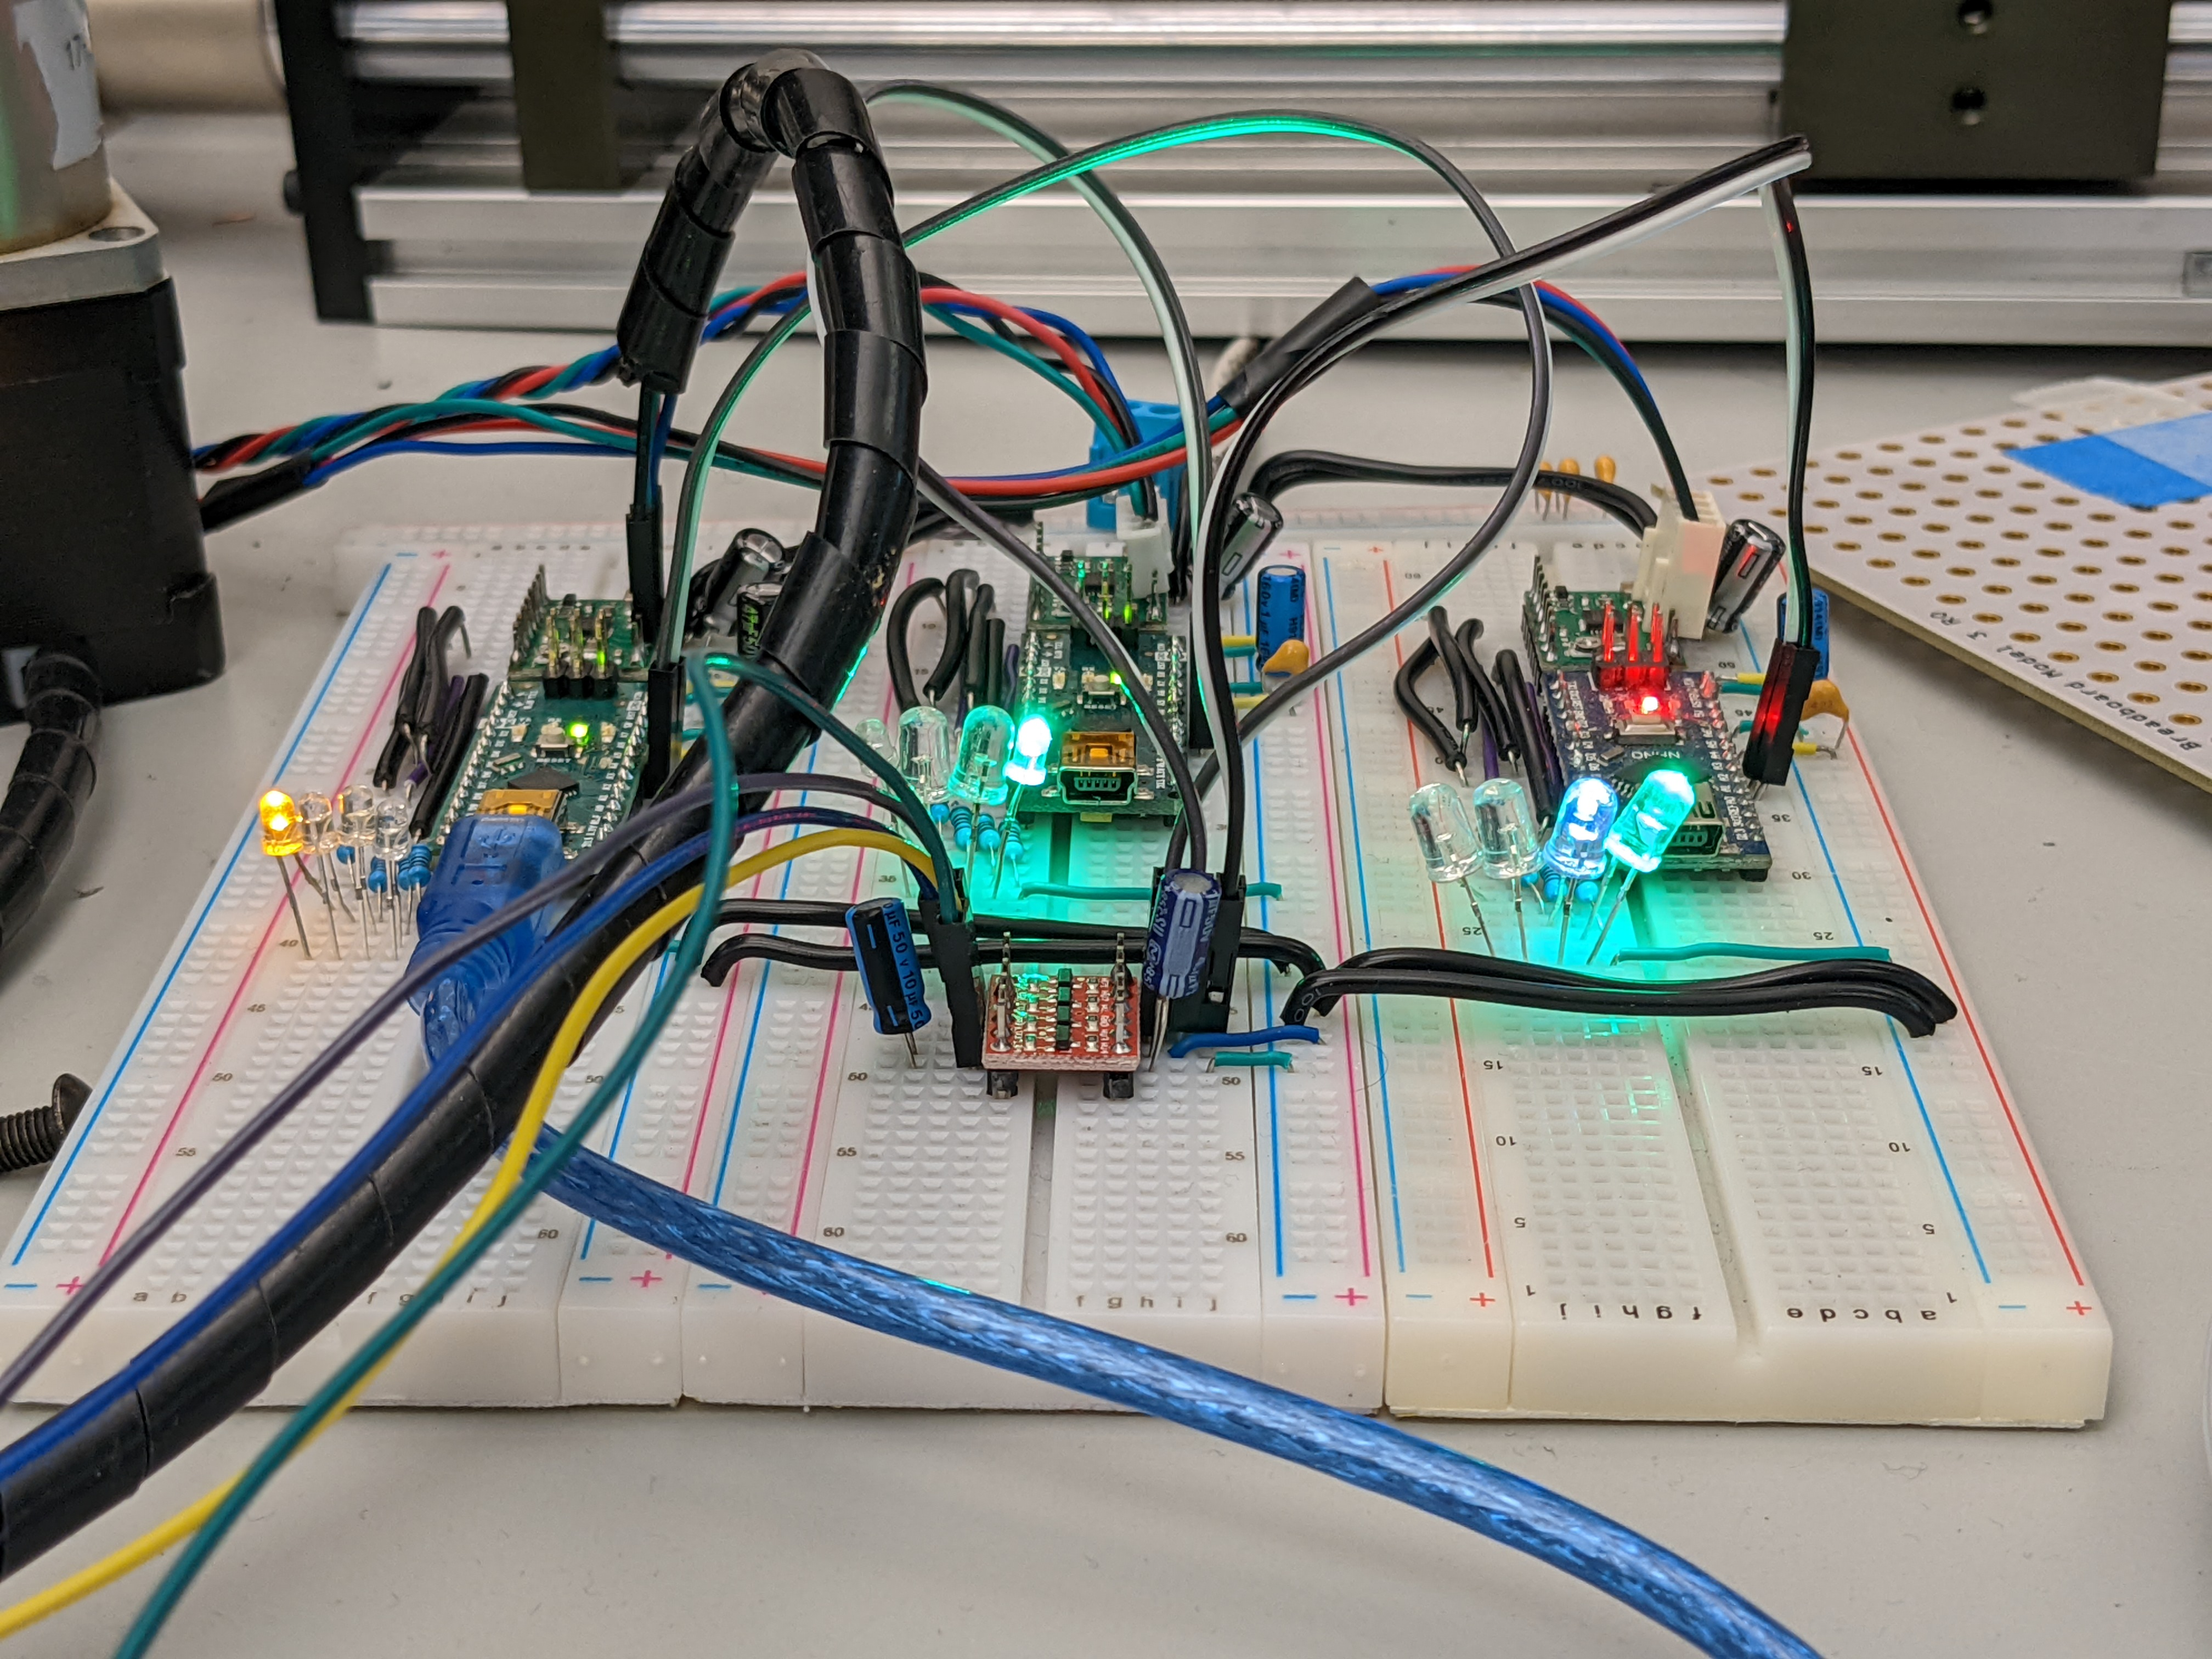
\includegraphics[width=7cm, height=5cm]{GUI_7_LED}
                \caption{LED Indicators during Run/Jog State}
                \label{fig:GUI7_L}
            \end{figure}
            
            Figure \ref{fig:GUI7}/\ref{fig:GUI9} also give information on the estop cursor. Figure \ref{fig:GUI7} shows the estop cursor on device one as "| ESTOP |" while Figure \ref{fig:GUI9} has its estop cursor at the bottom ( | ESTOP ALL? | ). The first figure will estop the device 1 only while the second figure will stop all of the devices if pressed. Figure \ref{fig:key_estop} shows the estop controls; they are using WASD but in a different order than the mode selection.   
            
            \begin{figure}[H]
                \centering
                \includegraphics[width=7cm, height=5cm]{GUI_9}
                \caption{Run Screen : E-Stop All Devices}
                \label{fig:GUI9}
            \end{figure}
            
            \begin{figure}[H]
                \centering
                \includegraphics[scale = 0.35]{KeySel_estop}
                \caption{Controls for E-Stop}
                \label{fig:key_estop}
            \end{figure}
            
            Figure \ref{fig:GUI10} shows an example of an estop event. The estop cursor is replaced with a | STOP'D | mark, the motor haulted, and the motor controller returns to the STANDBY state as seen in Figure \ref{fig:GUI10_L}
            
            \begin{figure}[H]
                \centering
                \includegraphics[width=7cm, height=5cm]{GUI_10}
                \caption{Run Screen : E-Stop Device \#2}
                \label{fig:GUI10}
            \end{figure}
            
            \begin{figure}[H]
                \centering
                \includegraphics[width=7cm, height=5cm]{GUI_10_LED}
                \caption{LED Indicator with E-Stop Event}
                \label{fig:GUI10_L}
            \end{figure}
            
            The hub controller communicates with each motor controller after the user has entered in the requested parameters. No motor controller hardware is the same and as such, each user request is checked my the motor controller to see if the hardware can produce the correct output. If the requested volumetric flow rate is too large for the hardware to output, an error message will appear (Figure \ref{fig:GUI12}) and the user will be prompted to enter new parameters. Other error codes exist: Figure \ref{fig:GUI14} is too small a Q value and Figure \ref{fig:GUI15} refers to the run time exceeding the fluid capacity of the syringe. 
            
            \begin{figure}[H]
                \centering
                \includegraphics[width=7cm, height=5cm]{GUI_12}
                \caption{Error Code : Too Large for Hardware to Output}
                \label{fig:GUI12}
            \end{figure}
            
            \begin{figure}[H]
                \centering
                \includegraphics[width=7cm, height=5cm]{GUI_14}
                \caption{Error Code : Too Small for Hardware to Output}
                \label{fig:GUI14}
            \end{figure}
            
            \begin{figure}[H]
                \centering
                \includegraphics[width=7cm, height=5cm]{GUI_15}
                \caption{Error Code : Too Long for Hardware to Run}
                \label{fig:GUI15}
            \end{figure}
            %\vspace*{-2.0in}
            
            After all devices have halted, the GUI screen will return to polling for the device run mode and all of the indicator LEDs will revert back to yellow. 
            %\vspace*{-1in}
        
        \subsubsection{Logic Flow}
            This subsection discusses the logic flow of the hub controller. The python code of this controller can be seen in Appendix \ref{Appendix:Code}. 
            %\vspace*{-0.5in}
            
            Looking at Figure \ref{fig:hub0}, the hub controller has four states that it operates in: START, DATAPULL, RUN, and RESET. The START state is written to do a few items: note which devices are active on the I2C bus, reset the motor controllers to their STANDBY state, and ask the user which run mode is proper for each device. After all active devices have selected a run mode, the hub transitions to DATAPULL. DATAPULL will prompt the user for data parameters ( volumetric flow rate Q, syringe radius, syringe capacity, duration, and motor direction) and send that data to the individual motor controllers. Should the user request be outside the operating range of the hardware, the motor controller will send back an error code that will be displayed on the GUI. The program will loop until all devices are error free and the system is ready to progress into the next state. The RUN state will turn on the stepper motors and poll for a stop condition. Should the user select an estop in the GUI or the motor controller reach its max time duration, the motor controller will shut off the motor and the hub will reset for that device. After all devices have reached a stop condition, the hub will proceed to the RESET state to clear all user parameters in the hub/motor controllers. The hub will return to the START state and STANDBY in the motor controllers. 
            
            It should be noted that the GUI referenced in the previous subsection is the same here and can be referenced as such. 
            
            \begin{figure}[H]
                \centering
                \includegraphics[width= 8cm, height = 13cm]{hub_L0}
                \caption{Top Level Flow Chart of Hub Controller}
                \label{fig:hub0}
            \end{figure}
            
            
        
    \subsection{Motor Controller}
        This subsection discusses an individual motor controller in the SMSS in three different sub-sub-sections. The first will discuss the characterization of the system, the second will map the control flow, and lastly there is a section about the I2C communication between the hub and motor controllers.
        
            \subsubsection{Plant Characterization}
                Starting with the syringe, the mechanical conversion that takes place in the syringe is as follows in Figure \ref{fig:q2v}. The volume of fluid displaced by the syringe plunger is proportional to the speed at which the plunger is moving. This plunger speed (V) is applied across the plunger's surface area, producing a volumetric flow \( \frac{m^3}{sec}\). This unit can be converted to \( \frac{L}{sec}\) with unit conversion.
                
                \begin{figure}[H]
                    \centering
                    \includegraphics[scale = 0.55]{syringe}
                    \caption{Components of a Syringe}
                    \label{fig:syringe}
                \end{figure}
                
                \begin{figure}[H]
                    \centering
                    \includegraphics[width= 8cm, height = 2.5cm]{Q_2_V}
                    \caption{Plant Conversion of Syringe}
                    \label{fig:q2v}
                \end{figure}
                
                
               After understanding how the linear velocity V is translated into a volumetric flow rate Q, lets discuss how the gearbox's RPM is converted into a linear velocity. Figure \ref{fig:rot2lin} illustrates how the RPM from the gearbox is translated to a linear velocity on the syringe plunger. The gearbox shaft is coupled to the screw rod at a 1 to 1 ratio; this segment does not require further analysis as no slip was witnessed. The interaction of the screw rod and the pillow block does however : the pillow block is attached to the frame of the ball screw kit and must be engaged with the screw rod to move. The helical spiral in Figure \ref{fig:helix} represents the screw rod that engages with the threaded bearing in the pillow block. The linear speed of the pillow block is dependant on the the rotational speed as well as a few factors. The position of a single particle on the helix is represented as r(t), with respect to time. 
               

               \begin{figure}[h]
                    \centering
                    \includegraphics[width= 8cm, height = 3cm]{rot_2_lin}
                    \caption{Translation of Angular Velocity to Linear Velocity}
                    \label{fig:rot2lin}
                \end{figure}
                
                \begin{figure}[h]
                    \centering
                    \includegraphics[width= 6cm, height = 5cm]{Images/Cylinder_coord.png}
                    \caption{Cylindrical Helix Model for Ball Screw}
                    \label{fig:helix}
                \end{figure}
                
                \begin{equation}
                    \begin{split}
                        Let\,\, r(t) = \rho \cos(\overrightarrow{\omega_g}t)\,\hat{\mathbb{A}}_x + 
                                        \rho \sin(\overrightarrow{\omega_g}t)\,\hat{\mathbb{A}}_y +
                                        \gamma \overrightarrow{\omega_g}t\,\hat{\mathbb{A}}_z \,\,\,\,\,\,\left [m\right]
                    \end{split}
                \end{equation}
                                
                Where \(\rho\) is the screw rod radius and \(\gamma\) is the rod's pitch. The rod's pitch is the z-axis distance between points of the same xy angle.
                
                To find the velocity of the particle with respect to time, the derivative of r(t) is taken.
                \begin{equation}
                    \begin{split}
                         \overrightarrow{v}(t) = \frac{d}{dt}\, r(t) \,\,\,\,\,\,\left [\frac{m}{s}\right]
                    \end{split}
                \end{equation}
                    

                \begin{equation}
                    \begin{split}
                        \scriptsize{
                        \overrightarrow{v}(t) = - \rho \overrightarrow{\omega_g} \sin(\overrightarrow{\omega_g}t)\,\hat{\mathbb{A}}_x + 
                        \rho \overrightarrow{\omega_g} \cos(\overrightarrow{\omega_g}t)\,\hat{\mathbb{A}}_y + 
                        \gamma \overrightarrow{\omega_g} \,\hat{\mathbb{A}}_z
                        \,\,\,\,\,\,\left [\frac{m}{s}\right]}
                    \end{split}
                \end{equation}
                
                Focusing attention on the Z-axis movement :
                
                \begin{equation}
                    \begin{split}
                        {\overrightarrow{v_z}(t)} &= \gamma \overrightarrow{\omega_g} \,\,\,\,\,\,\left [\frac{m}{s}\right] \\
                        \overrightarrow{\omega_g} &= \frac{{\overrightarrow{v_z}(t)}}{\gamma}
                        \,\,\,\,\,\,\left [\frac{rad}{s}\right] \\
                        {\overrightarrow{RPM}}_{gearbox}(t) &= \frac{2\pi {\overrightarrow{v_z}(t)}}{\gamma}
                        \,\,\,\,\,\,\left [\frac{Rev}{s}\right]
                    \end{split}
                \end{equation}
                
                The final equation relates the rotational speed of the gearbox to the linear velocity of the pillow block. Figure \ref{fig:rps_2_Q} is the plant of the system from this point. From here, relating individual steps of the stepper motor to the output RPS is the final step in characterizing the system. The STSPIN820 motor driver can output up to 256 microsteps, allowing the driver to further divide the input PWM freq at the cost of motor torque \cite{stepper_theory}. The stepper motor itself markets 200 steps per revolution; both motor step and the driver's microstep will alter the motor's speed. Figure \ref{fig:total_hard} depicts the addition of both step properties as well as the final representation of the hardware system.   
                
                \begin{figure}[H]
                    \centering
                    \includegraphics[width= 9.5cm, height = 4cm]{rps_2_Q}
                    \caption{Translation of Motor Speed to Flow Rate}
                    \label{fig:rps_2_Q}
                \end{figure}
                
                \begin{figure}[H]
                    \centering
                    \includegraphics[scale = 0.35]{total_hardware}
                    \caption{Complete Hardware Characterization of Pump}
                    \label{fig:total_hard}
                \end{figure}
                
                Working backward to find the appropriate frequency, \(f_{user}\) can be defined as : 
                \begin{equation}
                    \begin{split}
                        f_{user} &= X_m * \frac{400\pi N Q}{1000\gamma \pi r^2 }\\
                         &= X_m * \frac{2 N Q}{5\gamma r^2 }
                     \end{split}
                \end{equation}
                where N is the gear ratio, \(\gamma\) is the pitch of the ball screw, \(X_m\) is the microstep divisor, \(f_{user}\) is the frequency derived from the user requested Q, and r is the radius of the syringe plunger.
                
                From experimentation, it was found that the minimum frequency the stepper motor should operate at or above is 120 Hz (\(f_{min} = 120Hz\)). With this standard, finding the proper microstep size is a simple equation : 
                
                \begin{equation}
                    \begin{split}
                        f_{user} &\geq f_{min}\\ 
                        X_m * \frac{2 N Q}{5\gamma r^2 } &\geq f_{min}\\
                        X_m &\geq \frac{f_{min}}{\frac{2 N Q}{5\gamma r^2 }}\\
                        \therefore X_m &\geq \frac{5 \gamma r^2 f_{min}}{2NQ}
                    \end{split}
                \end{equation}
                
                The range of Q is limited to the frequency range of the stepper motor and was found experimentally as well. Both maximum and minimum Q values would stall the stepper motor. It was also noticed that frequencies above and below the range could move the motor but not reliably. The reliable range is : 
                
                \[ Q \,\,\in \,\,[10n, 16\mu] \,\,\,\, \left [\frac{L}{sec} \right ]\]
                
            \subsubsection{\hl{Control Flow}}
                The individual pump/motor controllers have the same code structure but can have different hardware parameters (syringe radius, ball screw radius, etc). Moreover, each controller can be placed into a I2C mode - the hub controller will dictate the flow of user info, or in serial mode - the Arduino IDE serial terminal will prompt the user for information. It should be noted that the serial method is device specific and wont control more than one pump controller. The serial mode is also referred as manual mode because it is easy to tune parameters for an individual pump without the use of an additional controller. To use either mode, comment out the unused setting as in Figure \ref{fig:comments}. 
                
                Both modes of the motor controller use different communication protocols but are similar in state structure. Figure \ref{fig:motor0} represents the highest level of flow for the motor controller : 6 states that will continue to loop until power is cycled. The controller will start and stay in STANDBY until the controller has received a START/JOG request. After leaving, the controller will go in to either DATAPULL\_S (for timed duration) or DATAPULL\_J (for jog) to retrieve the hardware parameters from the user. This data can be from I2C or serial depending on which portion of code had been enabled. After checking for errors, the device will proceed to the appropriate RUN state. Once the device has received an ESTOP or time-dependent FINISH command, the device will reset all variables in ESTOP and proceed to wait in STANDBY. This top level is almost identical to the hub controller but has many lower level differences. 
                
                Lower level flow charting can be found in Appendix \ref{Appendix:Documents}.
                
                
                
                
                \begin{figure}[H]
                    \centering
                    \includegraphics[scale = 0.55]{comments}
                    \caption{Tool selection for the Motor Controller}
                    \label{fig:comments}
                \end{figure}
                
                
                \begin{figure}[H]
                    \centering
                    \includegraphics[scale = 0.45]{Top_level_ver1}
                    \caption{Top Level Flow Chart of Motor Controller}
                    \label{fig:motor0}
                \end{figure}
                
                
                
            \subsubsection{I2C Communication Between Controllers}
                The hub controller assumes the position of the main device with the pump controllers acting as sub devices. The sub devices don't communicate with each other; only the hub controller sends a receive (MOSI) or request (MISO) command. The hub controller is a raspberry pi,  which a logic high of 3.3V, and the pump controller, arduino nano, has a logic high of 5v. With a difference in logic level voltage, a bi-directional logic converter was used in order for the devices to communicate to each other without hardware damage. For simplicity, a Sparkfun MOSFET converter was used as seen in the Appendix \ref{Appendix:Documents} schematics. 
                
                The data sent and requested by the main controller was often over the single packet 255 bit limit. To overcome this, data packets are processed to handle numbers less than 16,777,215. This is done by sending factors that are multiplied by 256 as well as remainders that are summed with the total number. The trade off for this solution is the extra time it takes to transmit three extra packets of information.  
                
                
                If the number is large enough to fill the second factor,
                \[ Number = 256 * (256 Fact_2 + Remain_2) + Remain_1\]
                
                else :
                \[ Number = 256 Fact_1 + Remain_1\]
                
                where each variable above represents a single packet.
                

\section{Testing}
        This section outlines the process for verifying the engineering requirements (Table \ref{table:EngineeringReq}) of the SMSS. The financial requirement, keeping the SMSS under \$500 USD is verifiable by viewing the Bill of Materials in Appendix \ref{Appendix:Documents} Figure \ref{fig:BoM}. This requirement is met for this generation of the SMSS because the cost was under \$500 USD. 
        
        The second and third requirement will be validated in the next section below; the fourth requirement can be verified by noting the libraries and hardware used. The code (Appendix \ref{Appendix:Code}) that was used is open source online and the hardware is not locked by physical/digital means. Both Arduino and Raspberry Pi devices are designed to be altered down to the copper or the kernel. 
        
        The fifth requirement was verified visually by inserting different syringes into the housing. The recorded range of syringes was 1mL to 30mL, going beyond the requirement. 
        
        Requirement six, concerning 3 pump controllers, is also verified in the subsection below. That requirement requests an analysis of three separate devices and their output flow rate. 
        
        Requirement seven is the GUI requirement and it is met by viewing the hub controller section earlier on in the paper. 
        
        Requirement eight, requesting that the drive train and pump housing be 3D printed, has fallen short of its goal. The drive train is a metallic ball screw that must be metal for friction and wear purposes. 3D printing this piece would require additional work for a lesser component. The housing of the entire system has also yet to be 3D printed because the footprint of the SMSS will continue to decrease. It was not fit to enclose the entire system at this stage of prototyping. Printing a piece that hold the ball screw and syringe together has proved to be a value component in this stage of the SMSS. 
        
        The last requirement was also short of its goal. This generation of the SMSS was unable to integrate viable feedback in the system. Different feedback methods (potentiometers, resolvers, pressure sensors) were considered but were left out due to budget and time constraints. Without feedback, output data couldn't be produced and sent to the hub controller. 
        
    \subsection{Verification Method for Hardware}
        The output flow rate of the SMSS was measured with a LabSmith uProcess kit. This kit measures the pressure inside a CapTile cavity and was the only method used. To use this device properly, the user must setup the device as shown in Figure \ref{fig:verif_diagram} and note physical measurements of the differential tubing. This tube's inner diameter and length are important in translating the pressure measurement into a measured volumetric flow rate. While the SMSS is applying pressure on the plunger of the syringe, water is flowing through the filter and into the three-way CapTile. The uPOS senor then measures the pressure at its highest potential at the intersection in reference to the lowest potential point at the other end of the differential tube. The pressure across the differential tube is the measured result \( \triangle P   \,\,\,\, [kPa]  \). The change in pressure can be translated into a volumetric flow rate with the following equation. It should be noted that the GUI has Q in terms of nL/sec, hence the conversion to nL/s here.
        
        \begin{equation}
            \begin{split}
                \triangle P &= P_{meas} - P_{atm} \,\,\,\,\,\,\,\, [kPa] \\
                &\approx  P_{meas} - 1 \,\,\,\,\,\,\,\,\,\,\,\, [kPa]
            \end{split}
        \end{equation}
        
        
        \begin{equation}
            \begin{split}
                Q_{deriv} &= \frac{\pi \,\,(\triangle P) \,\,D^4}{128 \mu \,\,\mathbb{L}}  \,\,\,\,\left[\frac{m^3}{sec}\right]\\
                &= \frac{\pi \,\,(\triangle P) \,\,D^4}{128 \mu \,\,\mathbb{L}} * \frac{10^3 L}{m^3} * \frac{10^9 nL}{L} * \frac{10^3 Pa}{kPa} \,\,\,\,\left[\frac{nL}{sec}\right]\\
                \therefore &= \frac{\pi \,\,(\triangle P) \,\,D^4}{128 \mu \,\,\mathbb{L}} * 10^{15}  \,\,\,\,\left[\frac{nL}{sec}\right]
            \end{split}
        \end{equation}
        
        where
        \begin{itemize}
            \item \(\triangle P \) is the change is pressure measured by the uPOS (kPa)
            \item D is the inner diameter of the differential tube (m)
            \item \( \mu \) is the dynamic fluid viscosity of water at 21 C (Pa * sec)
            \item $\mathbb{L}$ is the length of the differential tube for which the pressure change takes place (m).
            \item \( Q_{deriv}\) is the volumetric flow rate derived from the change in pressure measurement (nL/sec). This variable will be compared with the Q value entered by the user in the GUI. 
        \end{itemize}
        
        \begin{figure}[H]
            \centering
            \includegraphics[scale = 0.55]{verif_diagram}
            \caption{Verification Model}
            \label{fig:verif_diagram}
        \end{figure}
        
    \subsection{Results}
        Using the setup in the sub-section above, a variety of nominal values were sampled. This method was used to experimentally find the operating range of the SMSS.
        
        \subsubsection{Ceiling of Q Range}
            The ceiling of an individual syringe pump was initially verified visually by witnessing the spin of the motor while coupled with a syringe. Later in the project, this was properly verified using the uProcess kit. All other values above 16\(\mu L\)/sec were not repeatable and ended up stalling the motor. It should be noted that this real max value of 16\(\mu L\)/sec is far below the set engineering requirement; below both the maximum and minimum requirement. Here are the results :
            
            \begin{table}[H]
                \renewcommand{\arraystretch}{1.3}
                \caption{Parameters of Ceiling Test}
                \label{table:test_param_ceiling}
                    \begin{center}
                        \begin{tabular}{|c|c|c|}
                            \hline
                            \bfseries Variable&
                            \bfseries Value&
                            \bfseries Unit
                            \\ \hline
                            
                            Syringe \#&
                            S1&
                            -
                            \\ \hline
                            
                            Motor \#&
                            M1&
                            -
                            \\ \hline
                            
                            Arduino \#&
                            A1&
                            -
                            \\ \hline
                            
                            Motor Controller \#&
                            STSPIN820&
                            -
                            \\ \hline
                            
                            Sensor&
                            uPOS250-T116&
                            -
                            \\ \hline
                            
                            Pipe Length \(\mathbb{L}\) &
                            0.0820&
                            m
                            \\ \hline
                            
                            Pipe Inner Dia D&
                            0.15&
                            mm
                            \\ \hline
                            
                            Dynamic Fluid Viscosity \(\mu\) &
                            0.000975 @ \(20^\circ\)C&
                            Pa*sec
                            \\ \hline
                            
                            
                            
                            Syringe Radius(GUI)&
                            11&
                            mm
                            \\ \hline
                            
                            Motor Direction&
                            Forward&
                            -
                            \\ \hline
                            
                        \end{tabular}
                    \end{center}
                \end{table}
                
                
                \begin{figure}[H]
                    \centering
                    \includegraphics[scale = 0.65]{Images/T2_coarse.jpg}
                    \caption{Coarse Measurement for Nominal Q : 16000 nL/sec}
                    \label{fig:T2_coarse}
                \end{figure}
                
                \begin{figure}[H]
                    \centering
                    \includegraphics[scale = 0.65]{Images/T2_fine.jpg}
                    \caption{Fine Measurement for Nominal Q : 16000 nL/sec}
                    \label{fig:T2_fine}
                \end{figure}
                
                Figure \ref{fig:T2_coarse} is the entire capture of processed data. There is an exponential rise to 16000 nL/sec and it holds around that number until the pump is turned off, near 150 seconds. The coarse figure appears to hit and stay on the nominal value however, Figure \ref{fig:T2_fine} shows differently. The same value lines are present but the measured result is oscillating around the nominal value. It should be noted that the water flowing out of the differential tube is jet-like and not droplets. 
                

                
        \subsubsection{Floor of Q Range}
        
            The smallest output was verified using the uProcess kit as well. The minimum engineering requirement (\( 100\mu L/sec\)) is higher than the experimental minimum (\( 10 nL/sec\)).
        
            \begin{table}[H]
                    \renewcommand{\arraystretch}{1.3}
                    \caption{Parameters of Floor Test}
                    \label{table:test_param_floor}
                        \begin{center}
                            \begin{tabular}{|c|c|c|}
                                \hline
                                \bfseries Variable&
                                \bfseries Value&
                                \bfseries Unit
                                \\ \hline
                                
                                Syringe \#&
                                S1&
                                -
                                \\ \hline
                                
                                Motor \#&
                                M1&
                                -
                                \\ \hline
                                
                                Arduino \#&
                                A1&
                                -
                                \\ \hline
                                
                                Motor Controller \#&
                                STSPIN820&
                                -
                                \\ \hline
                                
                                Senor&
                                uPOS250-T116&
                                -
                                \\ \hline
                                
                                Pipe Length \(\mathbb{L}\) &
                                0.0820&
                                m
                                \\ \hline
                                
                                Pipe Inner Dia D&
                                0.15&
                                mm
                                \\ \hline
                                
                                Dynamic Fluid Viscosity \(\mu\) &
                                0.000975 @ \(20^\circ\)C&
                                Pa*sec
                                \\ \hline
                                
                                
                                Syringe Radius(GUI)&
                                11&
                                mm
                                \\ \hline
                                
                                Motor Direction&
                                Forward&
                                -
                                \\ \hline
                                
                            \end{tabular}
                        \end{center}
                    \end{table}
                    
                \begin{figure}[H]
                    \centering
                    \includegraphics[scale = 0.60]{T4}
                    \caption{Measurement for Nominal Q : 10 nL/sec}
                    \label{fig:T4}
                \end{figure}
                
                \begin{figure}[H]
                    \centering
                    \includegraphics[scale = 0.65]{T5}
                    \caption{Measurement for Nominal Q : 70 nL/sec}
                    \label{fig:T5}
                \end{figure}
                
            Figure \ref{fig:T4} illustrates the volumetric flow output when the nominal Q value is 10 \(nL/sec\). The large pressure spikes seen aligned with droplets falling from the differential tube. When the droplet was building in size on the tip of the tube, the pressure would decrease. When the droplet fell, there was a large spike in pressure. It is difficult to say whether the pump could hit this nominal value accurately. 
            
            Figure \ref{fig:T5} has similar spikes to the previous figure but are less pronounced. The pressure spikes are related to the physical droplets as well; the syringe pump can hit this Q value reliably and largely stay within \( \pm 10 \% \) untuned.
            
            \begin{figure}[H]
                \centering
                \includegraphics[scale = 0.65]{T7}
                \caption{Special Measurement for Nominal Q : 70 nL/sec}
                \label{fig:T7}
            \end{figure}
            
            From this point, the data suggested that the exiting droplets were having an impact on the low Q data. Figure \ref{fig:T7} shows the same nominal flow request but with the differential tube under water in the collection dish. The measured data is far from the nominal value, using the assumption from equation (7), but the large spikes are smoother than the previous test. 
                
        \subsubsection{Additional Data within Range}
            Additional tests were made within the Q range described above. These tests are useful in understanding unforeseen problems in the system.
            
            \begin{table}[H]
                    \renewcommand{\arraystretch}{1.3}
                    \caption{Parameters of Additional Data}
                    \label{table:test_param_add}
                        \begin{center}
                            \begin{tabular}{|c|c|c|}
                                \hline
                                \bfseries Variable&
                                \bfseries Value&
                                \bfseries Unit
                                \\ \hline
                                
                                Syringe \#&
                                S1&
                                -
                                \\ \hline
                                
                                Motor \#&
                                M1&
                                -
                                \\ \hline
                                
                                Arduino \#&
                                A1&
                                -
                                \\ \hline
                                
                                Motor Controller \#&
                                STSPIN820&
                                -
                                \\ \hline
                                
                                Senor&
                                uPOS250-T116&
                                -
                                \\ \hline
                                
                                Pipe Length \(\mathbb{L}\) &
                                0.0820&
                                m
                                \\ \hline
                                
                                Pipe Inner Dia D&
                                0.15&
                                mm
                                \\ \hline
                                
                                Dynamic Fluid Viscosity \(\mu\) &
                                0.000975 @ \(20^\circ\)C&
                                Pa*sec
                                \\ \hline
                                
                                
                                Syringe Radius(GUI)&
                                11&
                                mm
                                \\ \hline
                                
                                Motor Direction&
                                Forward&
                                -
                                \\ \hline
                                
                            \end{tabular}
                        \end{center}
                    \end{table}
            
            \begin{figure}[H]
                \centering
                \includegraphics[scale = 0.65]{T8}
                \caption{Measurement for Nominal Q : 1000 nL/sec}
                \label{fig:T8}
            \end{figure}
            
            \begin{figure}[H]
                \centering
                \includegraphics[scale = 0.65]{T9}
                \caption{Special Measurement for Nominal Q : 5000 nL/sec}
                \label{fig:T9}
            \end{figure}
            
            Figure \ref{fig:T8} is additional data within the Q range. There are inconsistencies between 200 and 300 seconds while running the system naturally. Figure \ref{fig:T9} is another example of inconsistencies : the large dips between 200 - 300 seconds are the outcome motor failure. For one reason or another, the motor was stalling during testing, emitting a large hum and vibration. The cause for this is still unknown and output returns to the typical pattern after this event.
        
    \subsection{Analysis}
        After viewing the data, there is confidence that the pump system can achieve nominal rates within 70-16000 nL/sec, but a few problems have to be addressed. The measurement method used needs further investigation into the droplet phenomenon: does surface tension or falling droplets have an effect on low Q output? One correction could be to record data with the exit tubing under water; further testing is needed. 
        
        Other issues came from the 3D printed parts attached to the ball screw assembly: the amount of flex in these parts gave inaccurate readings for the initial round of tests. There were re-prints of existing parts with higher infill percentages as well as newly drafted parts that were over engineered to avoid flexing under pressure. The original set of prints did end up breaking over time and were recorded deafening the pressure data as their internal structure began to fail. It would be recommended to replace the existing 3D printed parts with materials that has little flex. 
        
        Another issue came from the motor or motor controller: there were periods where the motor struggled to output the correct frequency. This can be seen in the data in Figure \ref{fig:T9} as a large trough in the blue measured data. More testing is required to identify the root of this problem. 
        
        The idea of fine tuning the motor controllers was conceived early in the planning phase of the project but ended up not happening. It was decided that digitally tuning the controller before addressing the other mechanical / data validation problems would not be the best course of action. The error measured in the data was also above nominal in the lower Q values while below in higher values, making the tuning process more than a simple offset of frequency. 
        
        It should be noted that the range of Q dictated by the engineering requirements was not met : the individual pumps that comprise the SMSS are capable of nano-liter or micro-liter flow rates but not milliliter. A future re-assessment of the engineering requirements is needed in order to confirm that the smaller range is beneficial. Fortunately customer Dr Hawkins has expressed that the finer Q range is beneficial.

\section{Conclusion}

    This generation of the Smart Motor Syringe System demonstrated several new additions to this ongoing project while getting closer to a smooth, nominal volumetric flow rate. The new additions include but are not limited to : the introduction of a hub controller, a simple GUI, and multiple configuration setting for three complete motor controllers. 
    
    The hub controller and GUI were successful in directing the user's requests into viable data across all three devices. The user can control up to three devices, run each device manually or timed, get real time error codes, and emergency stop each device individually or all together. While the code has not been exhausted of all edge case bugs, there are still some underlying issues to address. For future endeavors, the python code written can be improved with more modular-based function scripting and the removal of most global variables in the code. Both of these items would improve the readability of the code and potentially increase the performance time. Communication between devices was also witnessed to be slower than initially thought, taking up to 100ms per transmission. Adjusting the I2C speed on both hub and motor controller unfortunately introduced more errors.
    
    Looking at the individual motor controllers, each device performed close to the nominal requested Q. Most of the measured volumetric flow rates came within a 5\% tolerance and demonstrated a finer accuracy than previously prescribed in the initial engineering requirements. That being said, there were considerable items that needed addressing. There were unforeseen motor stalls mid-test as well as large pressure spikes when measuring small Q values. This observation suggests that there should be a different testing setup that prevents droplets from forming on the differential tubing. Lastly, the use of 3D printed parts became a problem and contributed to a number of accuracy errors early on. It is strongly recommendation to replace all of the printed parts with metal or a material that doesn't flex. Only after designing parts that were either over-engineered and/or over-filled was there little dampening/delay in the system.
    
    Beyond the existing technology presented in this report, there are some short and long term endeavors. Better power connectors for the motor supply are an immediate upgrade that would reduce some uncertainty in troubleshooting the stepper motors. A feedback loop was a short term goal and engineering requirement that did not take off due to time and financial constraints. A feedback loop for each syringe pump would allow better control of the motor controllers while providing logging data to the hub controller. Additional output signals were a short term goal that was cut as well. Instead of the single step function output, Dr. Hawkins requested a ramping output with the potential for other wave forms. This item was eventually cut due to time constraints. A Long term goal for this project includes a PCB design to reduce the project's footprint.
    




% if have a single appendix:
%\appendix[Proof of the Zonklar Equations]
% or
%\appendix  % for no appendix heading
% do not use \section anymore after \appendix, only \section*
% is possibly needed

% use appendices with more than one appendix
% then use \section to start each appendix
% you must declare a \section before using any
% \subsection or using \label (\appendices by itself
% starts a section numbered zero.)
%


\appendices
\section{Impact Analysis of Senior Project}
    \label{Appendix:Impact}
    \textbf{
    {\-\hspace{0cm} Project Title : Smart Motor Syringe System \\
    Student Names : Connor Wilson \\
    Advisor’s Name : Ben Hawkins
    }
    }
    \subsection{Summary of Functional Requirements}
        The Smart Motor Syringe System is a syringe pump that aims to autonomously output
        multiple flow rates and provide the user with research-grade log data. It will be using three modular syringe pumps inside the system to administer three separated fluids. This system will be cost effective by utilizing open source hardware and software while providing medical grade flow rate tolerances.
    
    \subsection{Primary Constraints}
        The primary constraints of the SMSS include an absence of feedback, proprietary equipment, and budget. The absence of a feedback loop places a large risk on the system should part of the system change. The lack of custom equipment is also a constraint because the user can introduce a syringe or controller that is not well adapted to the existing SMSS system. Calibration would be required. Lastly, budget is a constraint because there cannot be high quality parts or application specific components without going over budget.
    
    \subsection{Economic}
        \begin{itemize}
            \item Human Capital :
            The SMSS will create jobs in engineering, manufacturing, sales, and marketing. The SMSS could have an international presence should the ideal company see growth opportunities overseas.
            
            \item Financial Capital :
            The SMSS is designed to perform a highly complex task for under market value. The open-source technology in this device will provide a large margin of overhead and profit while saving the customer a portion as well. The financial capital is also aimed at potential investors as the product grows into a company.
            
            \item Natural Capital :
            While the SMSS is made from non-renewable parts that cannot be viably broken down into raw resources, the SMSS components can be re-purposed very easily. Most of the components inside the SMSS are stand alone devices, like the Raspberry Pi or the Arduino Nano, that can be used for other projects. A 3D printed housing case can also be broken down in a PLA/ABS foundry much easier than a complex polyethylene injection mold.
                
            \item Cost and Timing : 
            The cost of the SMSS is broken down into assembly and validation. Since most of the manufacturing is done by the component sellers (Raspberry and Arduino), most of the time and cost spent in manufacturing is assembly. Validation on the other hand will require large sets of unit testing and calibration. This portion can easily be \$100 per product. Overall, as more testing and assembly turn to automation, the less spent on cost and time.
            
        \end{itemize}
        
        \begin{table}[H]
                \renewcommand{\arraystretch}{1.3}
                \caption{Expected Cost/Revenue if Manufactured on a Large Scale}
                \label{table:costs}
                    \begin{center}
                        \begin{tabular}{|c|c|c|}
                            \hline
                            
                            \bfseries If Manufactured&
                            \bfseries Units&
                            \bfseries Reasoning
                            \\\hline
                            
                            Units per year& 
                            200&
                            \makecell[l]{This is the initial\\
                                         market before\\
                                         appealing to the\\
                                         average consumer}
                            \\\hline
                            
                            \makecell{Manufactur-\\ing  Cost}&
                            \$400&
                            \makecell[l]{Number includes\\
                                         material, parts,\\
                                         labor, and  re-\\
                                         occurring valid-\\
                                         ation}
                            \\\hline
                            
                            \makecell{Purchase Price}&
                            \$500 &
                            \makecell[l]{Minimum Viable\\
                                         Product}
                            \\ \hline
                            
                            Profit per year&
                            \$10,000&
                            Estimated
                            \\ \hline
                            
                            \makecell{Operating cost\\ for user}&
                            \makecell[l]{\$200 USD for power\\
                                         \$ 40 for annual care}&
                            \makecell[l]{Device requires \\
                                         power and requires\\
                                         regular service for\\
                                         lubricated parts.}
                                         
                            \\ \hline
                            
                            
                        \end{tabular}
                    \end{center}
                \end{table}
        
    
    \subsection{Manufacturing}
        The SMSS will require a separate system for hardware assembly and validation along with software. Beyond the physical, validation testing and calibration will need to be performed on each unit as part of strict quality control. If the unit is sold as a kit, the open source hardware and software will be provided and the quality assurance will be left up to the user.
    
    \subsection{Environmental Impact}
        The SMSS will have a notable impact on the environment including significant power consumption, material consumption, and end-of-life disposal. The power consumed by this unit will add further demand for electricity and will not have a power saving feature due to its critical performance features being the minimum viable product. 3D printed shells will also require a lot of power from the grid. 
        
        Beyond power consumption, the SMSS will require large refinement of materials in order to make the components. This includes silicon for chips as well as precious metals that are in high demand. Chip shortages brought on by COVID-19 are also brought into play as manufacturers seek out unsavory alternatives for refined materials.
        
        This refinement also makes this product hard to recycle and reclaim. Stripping this project back into its separated forms will require a large amount of processing and possibly toxic chemicals that can cause damage to organic life. This includes the ABS printing filament.
    
    \subsection{Sustainability}
        \begin{itemize}
            \item {\bfseries Issues maintaining the complete device or system}
                The SMSS relies on the functionality of multiple micro-controllers, stepper motors, ball screws, and power converters. Fluids in the syringe could cause potential harm to the electrical components . Physical damage or build-up of particles along the drive train could cause potential strain and damage to the system, shortening the lifespan of the product.
                
                The SMSS is also an open source project, allowing the user to replace commercial hardware components and reprogram them using an online database (Github) of code.
                
            \item {\bfseries How the project impacts the sustainable use of resources}
                The SMSS does use electronic hardware that is hard to recycle but is easy to replace or reuse. It uses open source hardware/software and can be purchased, maintained, or re-purposed should the user no longer use the SMSS as intended.
            \item {\bfseries Upgrades that would improve the design of the project}
                Calibration kits and negative feedback are two endeavors that would greatly improve the performance and reliability of the SMSS. The calibration kits would allow the user to ensure the precision/accuracy rates are correct as the system ages. Tuning software parameters with the calibration kit could potentially save the user money. Feedback compensation is another idea that would allow the system to perform better and hold tighter tolerances.
            \item {\bfseries Challenges associated with upgrading the design}
                When upgrading the SMSS, it is important to take into account the customer base. If the customer is fluent in open source code/hardware, then applying updates through Git is likely the course of travel. Should the SMSS reach a launch data through the progress of others, it could potentially be up-gradable without pulling code requests. 
            
                The hardware will be easy to upgrade in the early prototype phases until a release date. These upgrades are not limited to those in the conclusion. 
        \end{itemize}
    
    \subsection{Ethical}
        The SMSS is an open source syringe pump that has a few concerns. First, having a medical device with potential security risks can cause a few issues and benefits. The security risks involved with open source are up for debate as some open source systems, such as Linux, are stronger because of their large user community involvement. That being said, the Raspberry and Arduino systems have security risks that could cause unforeseen consequences.

        Additional concerns arise if the user decides against using medical grade parts such as precision stepper motors or syringes. This option leaves the SMSS functionality up to the user should they void.

        Using this technology to intentionally cause harm goes against my personal ethics. Misusing or misdiagnosing concentrations or flow rates into an organism is also not safeguarded by this device and responsibility must be placed on the user.

    \subsection{Health and Safety}
        The SMSS is a medical device that could have grave consequences if system or user errors occur. Beyond validation, the user needs to fully understand the risk involved with injecting an organism with a particular fluid and concentration. Improper use of this equipment could also result in dire consequences. This could be a valid reason why this technology is not readily advertised to the public as it comes with a steep set of instructions for proper operation. Overall, this system could result in injury, serious harm, or even death if not used properly.

    \subsection{Social and Political}
        The political/social impact of the SMSS involves the right-to-repair. As
        companies turn away from patients, they deny consumers the right to repair their own products. By keeping proprietary technology secret, consumers are forced to seek third parties that specialize in reverse engineering. While the SMSS is open source, it does have a high operating standard. Should the SMSS become a viable and successful product, the open source angle of marketing could cause consumers to demand more legal freedoms with their products. That being said, consumers should have access to proper calibration to meet the SMSS’s bare engineering requirements.

        There are conflicts with having an option to repair the SMSS. As a prebuilt system, the SMSS will run as intended just as other devices on the market. However, repairing and altering this product should also be viable.
    

% you can choose not to have a title for an appendix
% if you want by leaving the argument blank


\newpage
\quad
\newpage

\section{Schematics}
    \label{Appendix:Schematic}
    \begin{figure}[H]
        \centering
        \includegraphics[scale = 0.35]{Images/fritz_layout.pdf}
        \caption{Hardware Layout of the SMSS}
        \label{fig:fritz_layout}
    \end{figure}
        
    \newpage
    \quad
    \newpage

    \begin{figure}[H]
        \centering
        \includegraphics[scale=0.5]{Images/fritz_schem.pdf}
        \caption{Schematic of the SMSS}
        \label{fig:fritz_schem}
    \end{figure}
    
    \newpage
    \quad
    \newpage
    
    \begin{figure}[H]
        \centering
        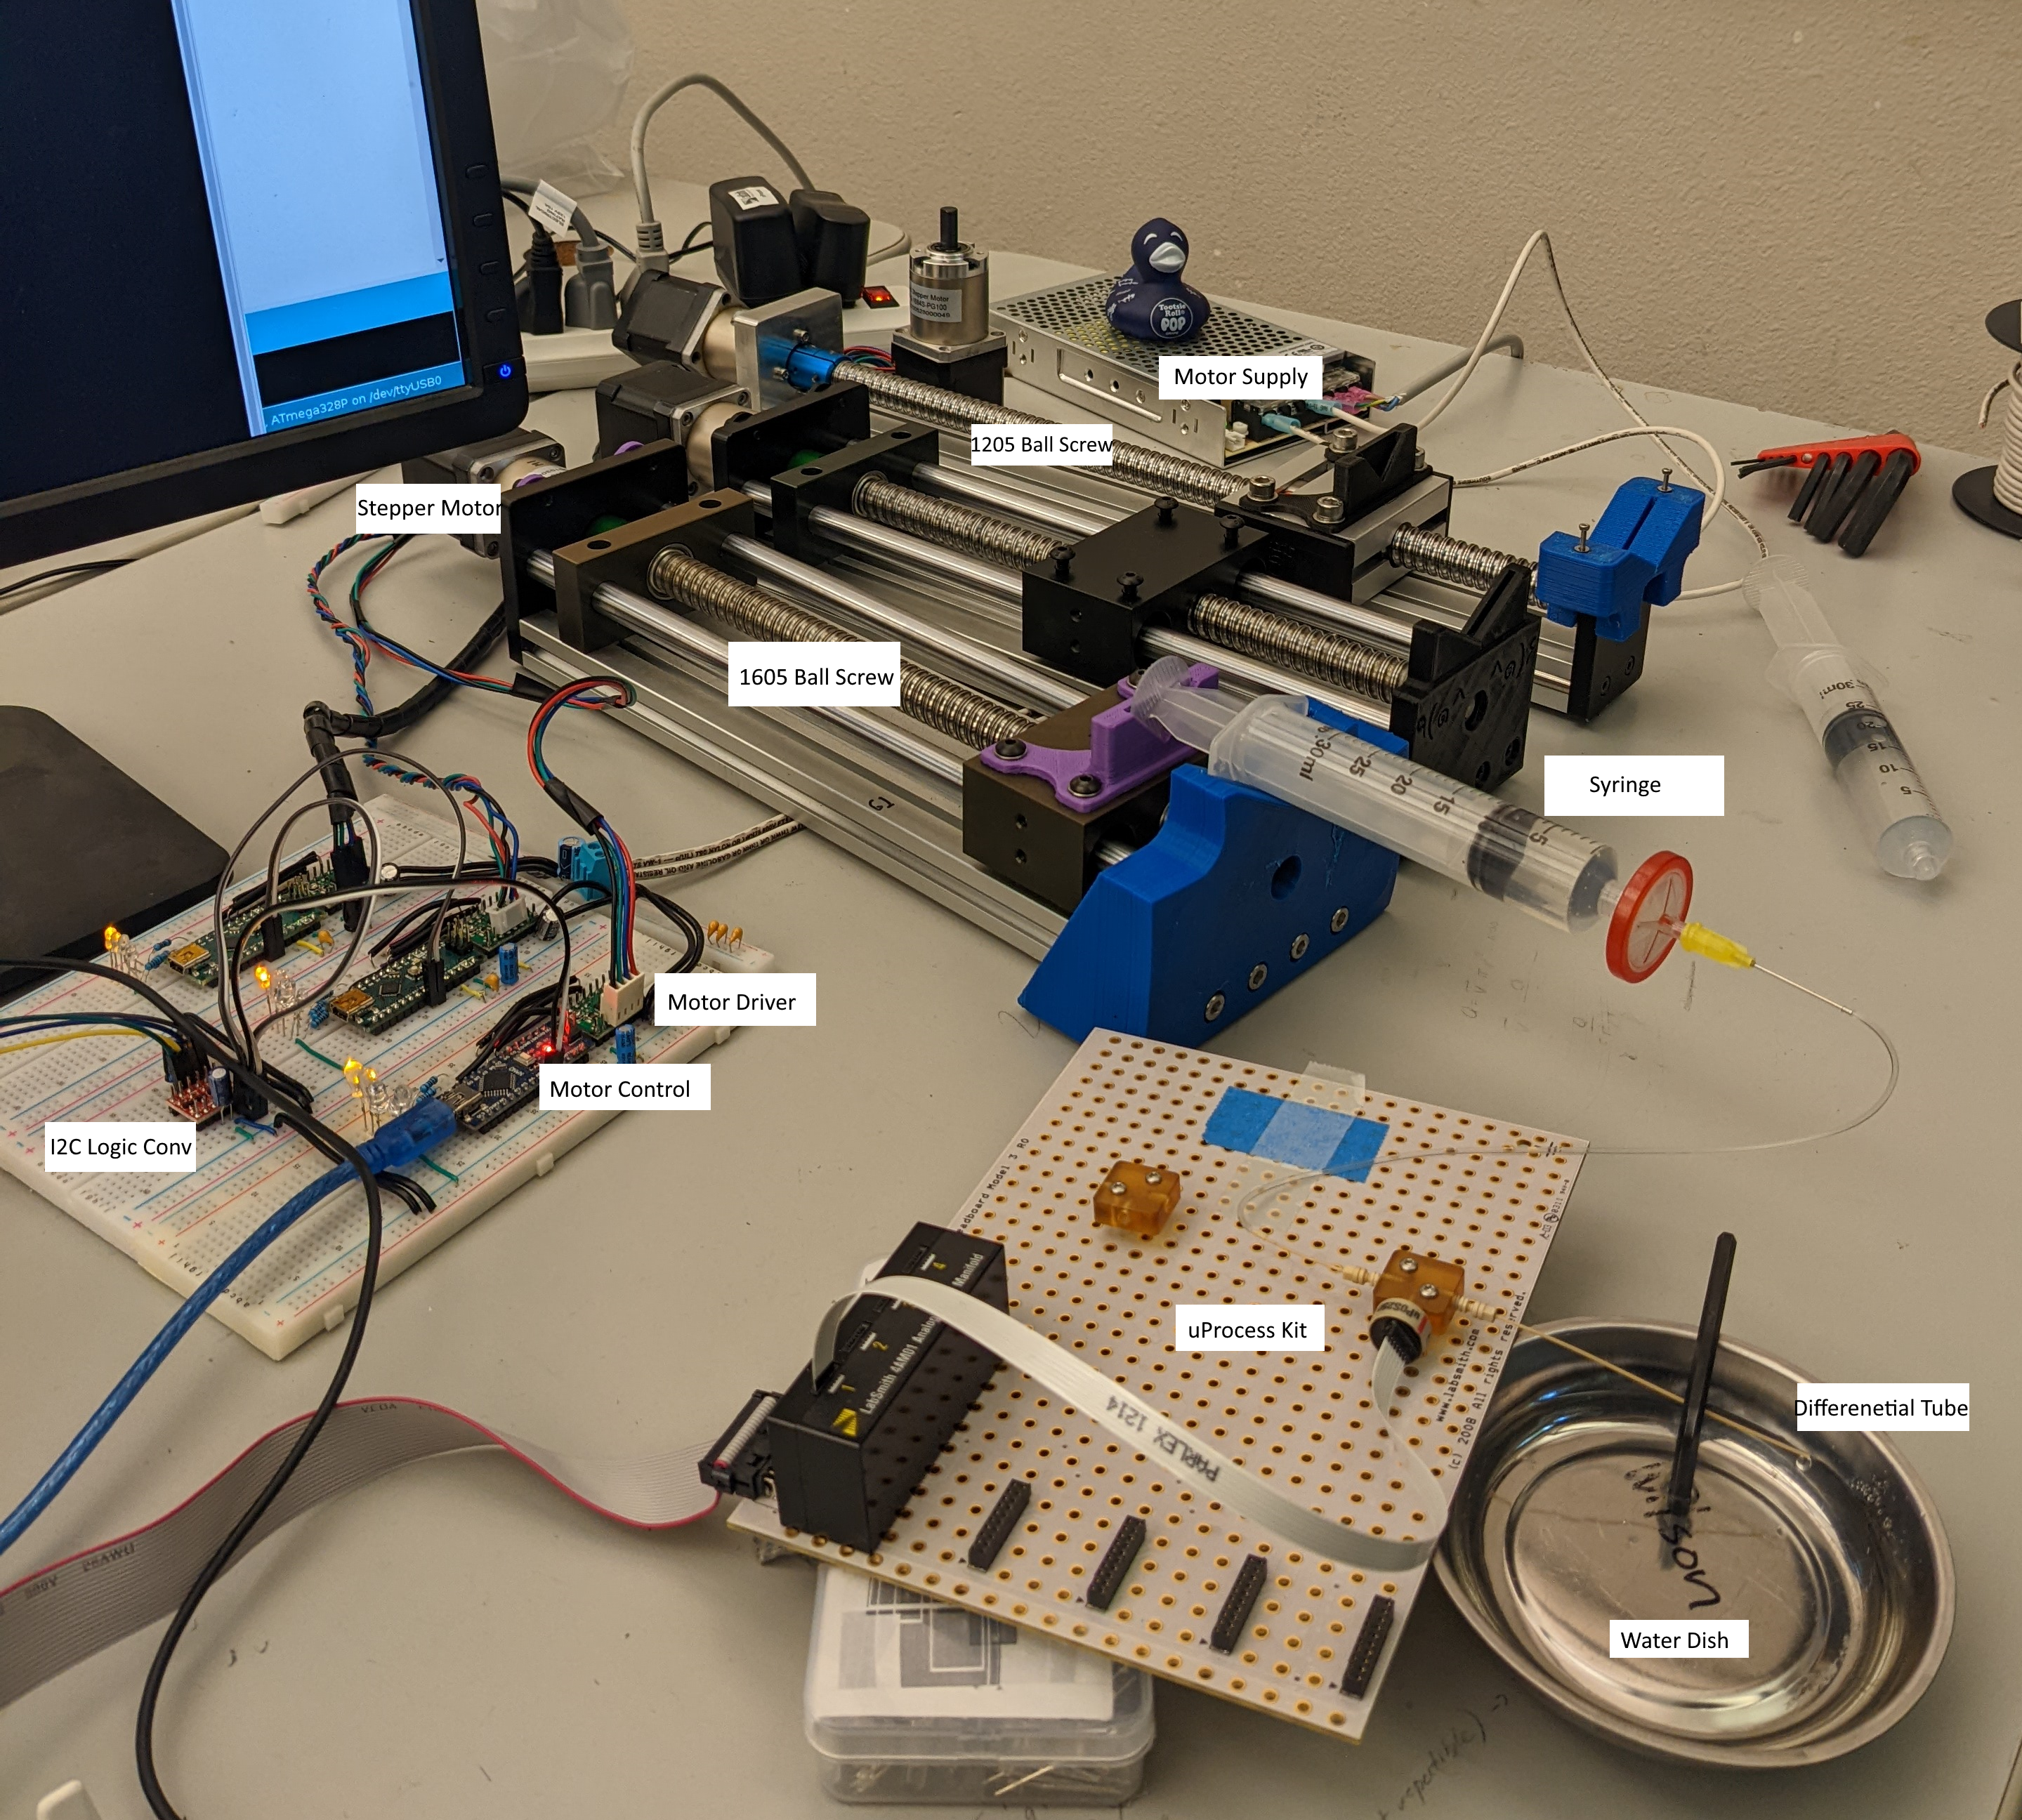
\includegraphics[scale=0.25, angle = 90]{Images/labstuff.png}
        \caption{Component Locations in the SMSS}
        \label{fig:physical}
    \end{figure}
    
    \newpage
    \quad
    \newpage



\section{Code}
    \label{Appendix:Code}
    \subsection{Motor Controller}
        \lstinputlisting[language=C++, caption= Motor Controller Code]{Motor_controller.ino}
        
    \newpage
    \quad
    \newpage
    

        
    \subsection{Hub Controller}
        \lstinputlisting[language=python, caption= Hub Controller Code]{Hub.py}
        
%\newpage
%\quad
%\newpage
\section{Additional Documents}
    \label{Appendix:Documents}
    \subsection{Business Model Graphic}
        \begin{figure}[H]
            \centering
            \includegraphics[width = 22cm, height = 18cm, angle=90]{Images/Business model.jpg}
            \caption{Business Model Graphic}
            \label{fig:business_sheet}
        \end{figure}
        
        \newpage
        \quad
        \newpage
        
    \subsection{Marketing Data Graphic}
        \begin{figure}[H]
            \centering
            \includegraphics[width = 22cm, height = 18cm, angle=90]{Images/Marketing model.jpg}
            \caption{Marketing Data Graphic}
            \label{fig:market_sheet}
        \end{figure}
        
        \newpage
        \quad
        \newpage
        
    \subsection{GANTT Chart}
        \begin{figure}[H]
            \centering
            \includegraphics[width = 18cm, height = 18cm]{Gantt}
            \caption{Gantt Chart for Current Version of the SMSS}
            \label{fig:Gantt}
        \end{figure}
        
        \newpage
        \quad
        \newpage
    
    \subsection{Bill of Materials}
        \begin{figure}[H]
            \centering
            \includegraphics[width = 18cm, height = 18cm]{BoM}
            \caption{Bill of Materials for Current Version of the SMSS}
            \label{fig:BoM}
        \end{figure}
        
        \newpage
        \quad
        \newpage
        
    \subsection{CAD Work}
        \begin{figure}[H]
            \centering
            \includegraphics[scale = 0.7]{Images/Small_flange_dwg.pdf}
            \caption{Flange Holder for Smaller 1205 Ball Screw}
            \label{fig:small_flange_dwg}
        \end{figure}
        
        \newpage
        \quad
        \newpage
        
        \begin{figure}[H]
            \centering
            \includegraphics[scale = 0.7]{backplate_winter2022}
            \caption{Flange Holder for Larger 1605 Ball Screw}
            \label{fig:large_flange_dwg}
        \end{figure}
        
        \newpage
        \quad
        \newpage
        
    \subsection{Motor Controller Flow}
        \begin{figure}[H]
            \centering
            \includegraphics[scale = 1]{Images/STANDBY_ver1.jpg}
            \caption{STANDBY Logic Flow for Motor Controller}
            \label{fig:STANDBY_mc}
        \end{figure}
        
        \newpage
        \quad
        \newpage
        
        \begin{figure}[H]
            \centering
            \includegraphics[scale = 1, angle=90]{Images/DATAPULL_J_ver1.jpg}
            \caption{DATAPULL\_J Logic Flow for Motor Controller}
            \label{fig:DATAPULLJ_mc}
        \end{figure}
        
        \newpage
        \quad
        \newpage
        
        \begin{figure}[H]
            \centering
            \includegraphics[scale = 0.75, angle=90]{Images/DATAPULL_S_ver1.jpg}
            \caption{DATAPULL\_S Logic Flow for Motor Controller}
            \label{fig:DATAPULLS_mc}
        \end{figure}
        
        \newpage
        \quad
        \newpage
        
        \begin{figure}[H]
            \centering
            \includegraphics[scale = 1.3]{Images/RUN_J_ver1.jpg}
            \caption{RUN\_J Logic Flow for Motor Controller}
            \label{fig:RUNJ_mc}
        \end{figure}
        
        \newpage
        \quad
        \newpage
        
        \begin{figure}[H]
            \centering
            \includegraphics[scale = 1]{Images/RUN_S_ver1.jpg}
            \caption{RUN\_S Logic Flow for Motor Controller}
            \label{fig:RUNS_mc}
        \end{figure}
        
        \newpage
        \quad
        \newpage
        
         \begin{figure}[H]
            \centering
            \includegraphics[scale = 1]{Images/STOP_ver1.jpg}
            \caption{STOP Logic Flow for Motor Controller}
            \label{fig:STOP_mc}
        \end{figure}
        
        
        
        
    \subsection{External Links}
        \begin{itemize}
            \item Github: github.com/Cwilson-WhisperingRock/SMSS22
        \end{itemize}
    
% use section* for acknowledgment
\section*{Acknowledgment}
    \label{Appendix:Ack}


    The author would like to thank
    \begin{itemize}
        \item Dr. Ben Hawkins for the guidance and knowledge to achieve success in a project such as this.
        \item Conrad Chan for putting forth amazing work for which this project stands on.
        \item My Fianc\'{e}e for humouring me in my engineering rambles. 
    \end{itemize}


% Can use something like this to put references on a page
% by themselves when using endfloat and the captionsoff option.
\ifCLASSOPTIONcaptionsoff
  \newpage
\fi



% trigger a \newpage just before the given reference
% number - used to balance the columns on the last page
% adjust value as needed - may need to be readjusted if
% the document is modified later
%\IEEEtriggeratref{8}
% The "triggered" command can be changed if desired:
%\IEEEtriggercmd{\enlargethispage{-5in}}

% references section
\bibliographystyle{ieeetr}
\printbibliography

\end{document}


